% Compile with XeLaTeX or Tectonic: tectonic How-an-LLM-Works.tex
\documentclass[11pt,a4paper]{article}
\usepackage{iftex}
\ifPDFTeX
  \usepackage[utf8]{inputenc}
  \usepackage[T1]{fontenc}
  \usepackage{lmodern}
\else
  \usepackage{fontspec}
\fi
\usepackage[margin=2.4cm]{geometry}
\usepackage{amsmath,amssymb}
\usepackage{microtype}
\usepackage{parskip}
\usepackage{graphicx}
\usepackage{float}
\usepackage[font=small,labelfont=bf]{caption}
\usepackage{array,booktabs,longtable}
\usepackage{xcolor}
\usepackage{listings}
\usepackage{needspace}
\usepackage[colorlinks=true,linkcolor=black,urlcolor=blue!55!black]{hyperref}

\definecolor{codebg}{gray}{0.965}
\definecolor{coderule}{gray}{0.82}
\lstset{
  basicstyle=\ttfamily\footnotesize,
  backgroundcolor=\color{codebg},
  frame=single,
  rulecolor=\color{coderule},
  framesep=5pt,
  xleftmargin=6pt,
  xrightmargin=6pt,
  columns=fullflexible,
  keepspaces=true,
  upquote=true,
  breaklines=true,
  breakindent=18pt,
  showstringspaces=false,
  keywordstyle=\color{blue!60!black},
  commentstyle=\color{black!55},
  stringstyle=\color{green!35!black},
  aboveskip=8pt,
  belowskip=8pt,
}
\setcounter{tocdepth}{1}
\setlength{\LTpre}{6pt}
\setlength{\LTpost}{8pt}
\newcommand{\vs}{\textvisiblespace}
\newcommand{\code}[1]{\texttt{#1}}
\raggedbottom

\title{How an LLM Works,\\Through the Small-GPT Code}
\author{}
\date{3 November 2026}

\begin{document}
\maketitle


An LLM is a function that reads tokens and gives a probability for every possible next token. Everything in this guide exists to make that one prediction good. It assumes you know Python, basic machine learning and basic deep learning, and it explains each idea with intuition, math and the real code from this repository.

\tableofcontents
\newpage

\section*{1. The big picture}
\phantomsection
\addcontentsline{toc}{section}{1. The big picture}

An LLM does one thing again and again: given the tokens so far, it scores every token in its vocabulary as the next one. Give the trained 24M model in this repository the words “Once upon a time, there was a little”. It returns a probability for all 4,096 of its tokens, and these are the highest:

{\small
\begin{longtable}{@{}>{\raggedright\arraybackslash}p{\dimexpr 0.400\linewidth-2\tabcolsep\relax}>{\raggedright\arraybackslash}p{\dimexpr 0.600\linewidth-2\tabcolsep\relax}@{}}
\toprule
\textbf{Next token} & \textbf{Probability} \\
\midrule
\endhead
girl & 45.1\% \\
boy & 30.1\% \\
dog & 5.5\% \\
bird & 2.4\% \\
cat & 1.3\% \\
\bottomrule
\end{longtable}
}

Training makes these probabilities match real text. Writing text means picking one token from this list, adding it to the input and asking again. Grammar, names and story shape all come from getting this one prediction right.

\begin{figure}[H]
\centering
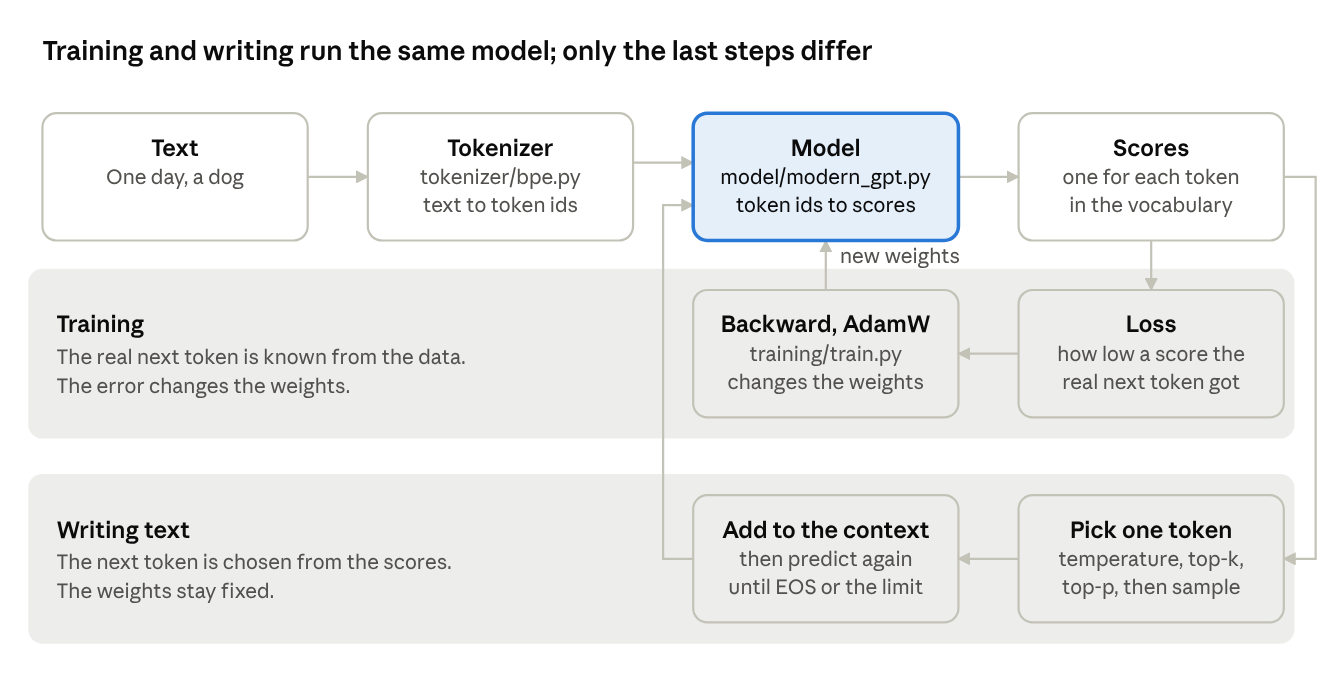
\includegraphics[width=\linewidth]{how-an-llm-works-figures/pipeline.png}
\caption{The path through this repository, for training and for writing text}
\end{figure}

The top row always runs the same way. Training continues through the middle band, and writing continues through the lower band.

\subsection*{Why a neural network and not a table of counts}
\phantomsection
\addcontentsline{toc}{subsection}{Why a neural network and not a table of counts}

A table cannot store this. With 4,096 tokens and 768 tokens of context, there are $4096^{768}$ possible contexts, so nearly every context is new. The network must learn patterns that carry over to contexts it has never seen.

The simplest table looks only at the previous token. On these stories it reaches a loss of 3.98, while the 24M network reaches 1.11. Section 10 explains that number.

\subsection*{Where each step lives}
\phantomsection
\addcontentsline{toc}{subsection}{Where each step lives}

The code is public at \href{https://github.com/Jannatul-Naim/small-GPT-Model}{github.com/Jannatul-Naim/small-GPT-Model}, and all paths in this guide are relative to it.

{\small
\begin{longtable}{@{}>{\raggedright\arraybackslash}p{\dimexpr 0.166\linewidth-2\tabcolsep\relax}>{\raggedright\arraybackslash}p{\dimexpr 0.407\linewidth-2\tabcolsep\relax}>{\raggedright\arraybackslash}p{\dimexpr 0.428\linewidth-2\tabcolsep\relax}@{}}
\toprule
\textbf{Step} & \textbf{File} & \textbf{Main names} \\
\midrule
\endhead
Turn text into token ids & tokenizer/bpe.py & BPETokenizer: train\_words, encode, decode \\
Build the training files & dataset/large\_text.py & build, write\_tokens \\
The network & model/modern\_gpt.py & ModernGPT, TransformerBlock, GQAAttention, apply\_rope, RMSNorm, SwiGLU \\
Model sizes and settings & training/config.py & CONFIGS, learning\_rate, batch\_size \\
Training loop & training/train.py & batch, lr, make\_optimizer, main \\
Scoring a saved model & evaluation.py & main \\
Writing text & model/modern\_gpt.py, generation/generate.py, web/server.py & generate, stream \\
\bottomrule
\end{longtable}
}

\subsection*{Two models appear in this guide}
\phantomsection
\addcontentsline{toc}{subsection}{Two models appear in this guide}

Real outputs come from the \code{medium} profile: 24.1M parameters, fully trained on TinyStories. Tensor shapes and parameter counts use the \code{large} profile: 184.6M parameters. Both run the same code.

Code in this guide is reformatted to save space, and any code shortened further is marked as simplified. Every number about these models was produced by running this code.

\section*{2. The tokenizer: text to integers}
\phantomsection
\addcontentsline{toc}{section}{2. The tokenizer: text to integers}

A model can only do math on numbers, so the tokenizer maps text to integer ids and back without losing anything. This repository uses BPE (byte pair encoding), which learns its pieces from the data by merging the most frequent neighbouring pair again and again.

\Needspace{10\baselineskip}
\subsection*{Why not characters or whole words}
\phantomsection
\addcontentsline{toc}{subsection}{Why not characters or whole words}

{\small
\begin{longtable}{@{}>{\raggedright\arraybackslash}p{\dimexpr 0.137\linewidth-2\tabcolsep\relax}>{\raggedright\arraybackslash}p{\dimexpr 0.255\linewidth-2\tabcolsep\relax}>{\raggedright\arraybackslash}p{\dimexpr 0.608\linewidth-2\tabcolsep\relax}@{}}
\toprule
\textbf{Unit} & \textbf{Vocabulary size} & \textbf{Problem} \\
\midrule
\endhead
Characters & About 100 & The context fills fast: 768 tokens hold only 768 characters \\
Whole words & Very large & Most words are rare, and a new word has no id at all \\
BPE pieces & 8,192 in the \code{large} model & None of these: common words stay whole and rare words split into known parts \\
\bottomrule
\end{longtable}
}

In the \code{large} model's story data, one token averages 4.25 characters. So a 768-token context holds about 3,260 characters.

\Needspace{10\baselineskip}
\subsection*{How ids are laid out}
\phantomsection
\addcontentsline{toc}{subsection}{How ids are laid out}

{\small
\begin{longtable}{@{}>{\raggedright\arraybackslash}p{\dimexpr 0.179\linewidth-2\tabcolsep\relax}>{\raggedright\arraybackslash}p{\dimexpr 0.821\linewidth-2\tabcolsep\relax}@{}}
\toprule
\textbf{Ids} & \textbf{Meaning} \\
\midrule
\endhead
0 to 3 & Special tokens: PAD, UNK, BOS, EOS \\
4 to 259 & One token for each of the 256 possible bytes \\
260 and up & Learned merges, in the order they were learned \\
\bottomrule
\end{longtable}
}

The vocabulary size is 4 + 256 + the number of merges, so 8,192 tokens means 7,932 merges. Every possible byte has a token, so any text can be encoded.

\subsection*{Step 1: split the text into word pieces}
\phantomsection
\addcontentsline{toc}{subsection}{Step 1: split the text into word pieces}

A regular expression cuts text into words, numbers, punctuation and spaces. A space stays attached to the word after it, so “ dog” and “dog” are different pieces.

\Needspace{7\baselineskip}
\begin{lstlisting}[language=Python]
# tokenizer/bpe.py
WORD_PIECE = re.compile(r" ?[^\W\d_]+| ?\d+| ?(?:[^\w\s]|_)+|\s+(?!\S)|\s+")

WORD_PIECE.findall("The dog's 3 balls,  and more!\n")
# ['The', ' dog', "'", 's', ' 3', ' balls', ',', ' ', ' and', ' more', '!', '\n']
\end{lstlisting}

Merges stay inside one piece, so a token never runs across two words. Training then only needs a count of the distinct pieces, which is why it can handle billions of tokens.

\subsection*{Step 2: learn the merges}
\phantomsection
\addcontentsline{toc}{subsection}{Step 2: learn the merges}

\begin{enumerate}
\item Write each piece as its bytes.
\item Count every neighbouring pair, weighted by how often its piece appears.
\item Merge the most frequent pair into one new token.
\item Repeat until the vocabulary is full.
\end{enumerate}

Here is the real \code{train\_\allowbreak{}words} on a tiny example: “ low” 5 times, “ lower” 2 times, “ newest” 6 times and “ widest” 3 times. The symbol \vs{} marks a space.

{\small
\begin{longtable}{@{}>{\raggedright\arraybackslash}p{\dimexpr 0.237\linewidth-2\tabcolsep\relax}>{\raggedright\arraybackslash}p{\dimexpr 0.263\linewidth-2\tabcolsep\relax}>{\raggedright\arraybackslash}p{\dimexpr 0.263\linewidth-2\tabcolsep\relax}>{\raggedright\arraybackslash}p{\dimexpr 0.237\linewidth-2\tabcolsep\relax}@{}}
\toprule
\textbf{Merge} & \textbf{Pair} & \textbf{New token} & \textbf{Count} \\
\midrule
\endhead
1 & e + s & es & 9 \\
2 & es + t & est & 9 \\
3 & \vs{} + l & \vs{}l & 7 \\
4 & o + w & ow & 7 \\
5 & \vs{}l + ow & \vs{}low & 7 \\
6 & \vs{} + n & \vs{}n & 6 \\
7 & e + w & ew & 6 \\
8 & \vs{}n + ew & \vs{}new & 6 \\
9 & \vs{}new + est & \vs{}newest & 6 \\
10 & \vs{} + w & \vs{}w & 3 \\
\bottomrule
\end{longtable}
}

\Needspace{10\baselineskip}
\begin{lstlisting}[language=Python]
# tokenizer/bpe.py, train_words (simplified: count updates left out)
words = [[OFFSET + b for b in piece.encode("utf-8")] for piece in piece_counts]

while len(self.merges) < target_merges:
    best_pair = most_frequent_pair()         # a heap keeps this fast
    new_id = OFFSET + BYTE_VOCAB_SIZE + len(self.merges)
    self.merges.append(best_pair)
    for index in pair_words.pop(best_pair):  # only pieces holding the pair
        words[index] = self._merge_pair(words[index], best_pair, new_id)
\end{lstlisting}

The intuition is compression. BPE began as a compression method, and each merge removes the most tokens it can at that moment. So frequent words end up as one token, and rare words stay as several.

\subsection*{Step 3: encode new text}
\phantomsection
\addcontentsline{toc}{subsection}{Step 3: encode new text}

To encode a piece, start from its bytes and keep applying the earliest-learned merge that fits. The order matters, because later merges were learned on top of earlier ones.

\Needspace{13\baselineskip}
\begin{lstlisting}[language=Python]
# tokenizer/bpe.py, _encode_piece (cache left out)
def _encode_piece(self, piece):
    tokens = [self.OFFSET + b for b in piece.encode("utf-8")]
    while len(tokens) > 1:
        ranked = [(self.merge_rank[pair], pair)
                  for pair in zip(tokens, tokens[1:])
                  if pair in self.merge_rank]
        if not ranked:
            break
        rank, pair = min(ranked)
        tokens = self._merge_pair(tokens, pair, self.OFFSET + self.BYTE_VOCAB_SIZE + rank)
    return tokens
\end{lstlisting}

With the tiny tokenizer above, words it never saw still work:

{\small
\begin{longtable}{@{}>{\raggedright\arraybackslash}p{\dimexpr 0.169\linewidth-2\tabcolsep\relax}>{\raggedright\arraybackslash}p{\dimexpr 0.186\linewidth-2\tabcolsep\relax}>{\raggedright\arraybackslash}p{\dimexpr 0.644\linewidth-2\tabcolsep\relax}@{}}
\toprule
\textbf{Text} & \textbf{Tokens} & \textbf{Why} \\
\midrule
\endhead
\vs{}newest & \vs{}newest & Seen often, so one token \\
\vs{}lowest & \vs{}low, est & Never seen, but built from known parts \\
\vs{}slow & \vs{}, s, l, ow & Only one merge fits \\
\bottomrule
\end{longtable}
}

The real 8,192-token tokenizer behaves the same way on real text:

{\small
\begin{longtable}{@{}>{\raggedright\arraybackslash}p{\dimexpr 0.436\linewidth-2\tabcolsep\relax}>{\raggedright\arraybackslash}p{\dimexpr 0.564\linewidth-2\tabcolsep\relax}@{}}
\toprule
\textbf{Text} & \textbf{Tokens} \\
\midrule
\endhead
Once upon a time, a little dog found a red ball. & Once, \vs{}upon, \vs{}a, \vs{}time, the comma, \vs{}a, \vs{}little, \vs{}dog, \vs{}found, \vs{}a, \vs{}red, \vs{}ball, the full stop (13 tokens) \\
\vs{}Transformer & \vs{}Tr, ans, form, er \\
\vs{}photosynthesis & \vs{}photos, y, nt, hes, is \\
\bottomrule
\end{longtable}
}

Its first merges were he, \vs{}t, \vs{}a, \vs{}s and \vs{}the. Its last merges include \vs{}muffins, \vs{}Captain and \vs{}conversation. So the most common pieces of English come first, and whole uncommon words come last.

\subsection*{Decoding}
\phantomsection
\addcontentsline{toc}{subsection}{Decoding}

Decoding looks up each token's bytes, joins them and reads the result as UTF-8. Each merge token is simply its two parts joined, so \code{\_\allowbreak{}symbol\_\allowbreak{}bytes} finds its bytes by recursion. All three real examples above came back exactly as they went in.

One token can hold only part of a multi-byte character. Decoded alone, it can show a replacement mark, even though the full sequence decodes correctly.

\subsection*{Two practical points}
\phantomsection
\addcontentsline{toc}{subsection}{Two practical points}

\begin{itemize}
\item \textbf{EOS matters.} The data build writes EOS (id 3) after every document, so the model learns to predict where a story ends. Without it, the model would never stop by itself.
\item \textbf{The tokenizer is part of the model.} The weights mean nothing with a different tokenizer, so each checkpoint stores \code{tokenizer\_\allowbreak{}sha256} and the trainer refuses a mismatch.
\end{itemize}

\section*{3. Training data: inputs and targets}
\phantomsection
\addcontentsline{toc}{section}{3. Training data: inputs and targets}

The training set is one long array of token ids. Each example is a window cut from it, and the target is the same window shifted one place along.

\subsection*{The file on disk}
\phantomsection
\addcontentsline{toc}{subsection}{The file on disk}

\code{dataset/\allowbreak{}large\_\allowbreak{}text.\allowbreak{}py} encodes every story and writes the ids to \code{train.\allowbreak{}bin} as 16-bit integers, with EOS after each story. The \code{large} model's file holds 1,147,643,766 tokens, about 2.3 GB.

The trainer opens it with \code{np.\allowbreak{}memmap}, which reads only the parts it touches. So the data does not need to fit in RAM.

\Needspace{12\baselineskip}
\subsection*{Cutting a batch}
\phantomsection
\addcontentsline{toc}{subsection}{Cutting a batch}

\begin{lstlisting}[language=Python]
# training/train.py
def batch(data, block, bs, device, generator=None):  # length check left out
    starts = torch.randint(0, len(data) - block - 1, (bs,), generator=generator).tolist()
    x = torch.stack([torch.from_numpy(np.asarray(data[i:i + block], dtype=np.int64)) for i in starts])
    y = torch.stack([torch.from_numpy(np.asarray(data[i + 1:i + block + 1], dtype=np.int64)) for i in starts])
    return x.to(device), y.to(device)
\end{lstlisting}

The only difference between \code{x} and \code{y} is the \code{+ 1}. Here is what that does to one short window:

{\small
\begin{longtable}{@{}>{\raggedright\arraybackslash}p{\dimexpr 0.200\linewidth-2\tabcolsep\relax}>{\raggedright\arraybackslash}p{\dimexpr 0.164\linewidth-2\tabcolsep\relax}>{\raggedright\arraybackslash}p{\dimexpr 0.164\linewidth-2\tabcolsep\relax}>{\raggedright\arraybackslash}p{\dimexpr 0.473\linewidth-2\tabcolsep\relax}@{}}
\toprule
\textbf{Position} & \textbf{Input x} & \textbf{Target y} & \textbf{What the model may look at} \\
\midrule
\endhead
0 & Once & \vs{}upon & Once \\
1 & \vs{}upon & \vs{}a & Once upon \\
2 & \vs{}a & \vs{}time & Once upon a \\
3 & \vs{}time & the comma & Once upon a time \\
\bottomrule
\end{longtable}
}

So one window is not one example. A 768-token window holds 768 separate predictions, from very short contexts up to long ones. Section 5 shows how a mask stops each position from seeing its own answer.

\Needspace{10\baselineskip}
\subsection*{How much data one step uses}
\phantomsection
\addcontentsline{toc}{subsection}{How much data one step uses}

{\small
\begin{longtable}{@{}>{\raggedright\arraybackslash}p{\dimexpr 0.419\linewidth-2\tabcolsep\relax}>{\raggedright\arraybackslash}p{\dimexpr 0.384\linewidth-2\tabcolsep\relax}>{\raggedright\arraybackslash}p{\dimexpr 0.198\linewidth-2\tabcolsep\relax}@{}}
\toprule
\textbf{Quantity} & \textbf{Calculation} & \textbf{Value} \\
\midrule
\endhead
Predictions in one forward pass & 8 windows $\times$ 768 tokens & 6,144 \\
Predictions in one optimizer step & 6,144 $\times$ 4 forward passes & 24,576 \\
Predictions in the whole \code{large} run & 24,576 $\times$ 93,400 steps & About 2.3 billion \\
Passes over the data & 2.3 billion $\div$ 1.15 billion tokens & 2.0 \\
\bottomrule
\end{longtable}
}

The code has no epochs, because each window starts at a random place. A pass here means “as many tokens as the data holds”, so some text is seen more than others.

A window can cross EOS and run into the next story. That is useful: the model sees what follows EOS, so it learns how stories begin.

\subsection*{Validation data}
\phantomsection
\addcontentsline{toc}{subsection}{Validation data}

\code{val.\allowbreak{}bin} is built from separate stories that training never uses. Its loss therefore shows how the model does on text it has not seen.

\code{evaluate} uses a fixed random seed, so every check scores the same windows. A change in validation loss then comes from the model, and not from a luckier sample. Each check scores 20 batches of 8 windows, which is 122,880 tokens.

\section*{4. Embeddings: tokens become vectors}
\phantomsection
\addcontentsline{toc}{section}{4. Embeddings: tokens become vectors}

An embedding gives every token a learned vector, so tokens used in similar ways can end up close together. Token ids cannot do this: id 607 is not “more” than id 478 in any useful sense.

\subsection*{The math}
\phantomsection
\addcontentsline{toc}{subsection}{The math}

The embedding is a matrix E with one row per token, V rows and d columns. Looking up a token means reading its row, which is the same as multiplying a one-hot vector by E.
\[
\mathbf{x}_i = \mathbf{E}^{\top}\mathbf{o}_i, \qquad \mathbf{E}\in\mathbb{R}^{V\times d}
\]

The matrix is an ordinary trainable parameter. In the \code{large} model it holds 8,192 $\times$ 1,024 = 8,388,608 numbers.

\Needspace{5\baselineskip}
\begin{lstlisting}[language=Python]
# model/modern_gpt.py
self.embedding = nn.Embedding(vocab_size, dim)   # in __init__
x = self.embedding(idx)                          # [B, T] becomes [B, T, dim]
\end{lstlisting}

The values start as small random numbers, drawn from a normal distribution with standard deviation 0.02. They mean nothing at first, and all their meaning comes from training.

\subsection*{What training put there}
\phantomsection
\addcontentsline{toc}{subsection}{What training put there}

This table reads the embedding matrix of the trained 24M model. It lists the closest tokens by cosine similarity, which is the dot product of two vectors after scaling each to length 1.
\[
\cos(\mathbf{a},\mathbf{b}) = \frac{\mathbf{a}\cdot\mathbf{b}}{\lVert\mathbf{a}\rVert\,\lVert\mathbf{b}\rVert}
\]

{\small
\begin{longtable}{@{}>{\raggedright\arraybackslash}p{\dimexpr 0.127\linewidth-2\tabcolsep\relax}>{\raggedright\arraybackslash}p{\dimexpr 0.873\linewidth-2\tabcolsep\relax}@{}}
\toprule
\textbf{Token} & \textbf{Closest tokens, with cosine similarity} \\
\midrule
\endhead
\vs{}dog & \vs{}cat 0.53, \vs{}dogs 0.49, \vs{}puppy 0.45, \vs{}Spot 0.41, \vs{}bird 0.38 \\
\vs{}red & \vs{}yellow 0.49, \vs{}blue 0.46, \vs{}pink 0.45, \vs{}green 0.42, \vs{}purple 0.40 \\
\vs{}three & \vs{}3 0.75, \vs{}four 0.59, \vs{}five 0.51, \vs{}two 0.49, \vs{}ten 0.46 \\
\vs{}ran & \vs{}runs 0.72, \vs{}run 0.65, \vs{}running 0.56, \vs{}walked 0.47, \vs{}raced 0.46 \\
\vs{}mom & \vs{}Mom 0.62, \vs{}mommy 0.62, \vs{}mother 0.55, \vs{}mum 0.55, \vs{}dad 0.54 \\
\vs{}happy & \vs{}glad 0.47, \vs{}happ 0.40, \vs{}excited 0.38, \vs{}happily 0.36, \vs{}proud 0.35 \\
\bottomrule
\end{longtable}
}

Nobody told the model what a colour or a number is. It grouped them because they appear in similar places in sentences, and sharing a similar vector helps prediction: what follows “dog” often follows “cat” too.

The grouping follows use, not dictionary meaning. \vs{}sad is also close to \vs{}happy, at 0.34, even though the meanings are opposite. Both fit the same slot: for “Lily was very”, the model gives \vs{}happy 40\% and \vs{}sad 18\%.

\subsection*{What embeddings cannot do}
\phantomsection
\addcontentsline{toc}{subsection}{What embeddings cannot do}

A token gets the same vector everywhere. It carries no position and no context, so “he” looks the same whoever it refers to. Adding that context is the job of the next section.

\section*{5. Attention: how tokens use each other}
\phantomsection
\addcontentsline{toc}{section}{5. Attention: how tokens use each other}

Attention lets each token build a new vector as a weighted average of information from earlier tokens. The weights are computed from the tokens themselves, so the model decides where to look.

\subsection*{The problem it solves}
\phantomsection
\addcontentsline{toc}{subsection}{The problem it solves}

Take the text “Tom saw a big cat. He was scared of the cat, so he”. To predict the next word, the model needs to know that “he” means Tom, and the vector for “he” alone cannot say that.

Older recurrent networks (RNNs) read one token at a time and squeeze everything into one fixed-size vector. Far-back details fade, and gradients must travel through every step. Attention lets any token look straight at any earlier token, and all positions can be computed at once.

\subsection*{The idea: a soft lookup}
\phantomsection
\addcontentsline{toc}{subsection}{The idea: a soft lookup}

A Python dict matches one key exactly and returns one value. Attention compares a query with every key and returns a mix of all the values, weighted by how well each key matched.

Each token's vector x goes through three learned linear maps:

{\small
\begin{longtable}{@{}>{\raggedright\arraybackslash}p{\dimexpr 0.158\linewidth-2\tabcolsep\relax}>{\raggedright\arraybackslash}p{\dimexpr 0.175\linewidth-2\tabcolsep\relax}>{\raggedright\arraybackslash}p{\dimexpr 0.667\linewidth-2\tabcolsep\relax}@{}}
\toprule
\textbf{Vector} & \textbf{Formula} & \textbf{Rough meaning} \\
\midrule
\endhead
Query q & q = $W_Q$ x & What this token is looking for \\
Key k & k = $W_K$ x & What this token can be found by \\
Value v & v = $W_V$ x & What this token hands over when chosen \\
\bottomrule
\end{longtable}
}

These meanings are only a way to think about it. The model is never told them, and it learns whatever maps lower the loss.

\subsection*{The math, one step at a time}
\phantomsection
\addcontentsline{toc}{subsection}{The math, one step at a time}

First, score how well token i's query matches token j's key. A large dot product means the two vectors point the same way.
\[
s_{ij} = \frac{\mathbf{q}_i \cdot \mathbf{k}_j}{\sqrt{d_k}}
\]

Second, block the future, so that a token can only look at itself and earlier tokens.
\[
s_{ij} = -\infty \quad \text{for } j > i
\]

Third, turn the scores into weights with softmax. The weights are positive and add up to 1, and a score of minus infinity becomes a weight of exactly 0.
\[
\alpha_{ij} = \frac{\exp(s_{ij})}{\sum_{l \le i} \exp(s_{il})}
\]

Fourth, take the weighted average of the values.
\[
\mathbf{o}_i = \sum_{j \le i} \alpha_{ij}\,\mathbf{v}_j
\]

All four steps fit in one matrix formula, which computes every token at once:
\[
\mathrm{Attention}(\mathbf{Q},\mathbf{K},\mathbf{V}) = \mathrm{softmax}\!\left(\frac{\mathbf{Q}\mathbf{K}^{\top}}{\sqrt{d_k}}\right)\mathbf{V}
\]

The repository calls PyTorch's optimized \code{F.\allowbreak{}scaled\_\allowbreak{}dot\_\allowbreak{}product\_\allowbreak{}attention}. These five lines give the same result, which was confirmed on the real Q, K and V of the 24M model:

\Needspace{7\baselineskip}
\begin{lstlisting}[language=Python]
scores = q @ k.transpose(-1, -2) / math.sqrt(q.size(-1))
mask = torch.tril(torch.ones(T, T, dtype=torch.bool))
scores = scores.masked_fill(~mask, float("-inf"))
weights = scores.softmax(dim=-1)
output = weights @ v
\end{lstlisting}

\subsection*{A worked example}
\phantomsection
\addcontentsline{toc}{subsection}{A worked example}

Take 3 tokens with $d_k$ = 2, and these small matrices. Each row is one token.
\[
\mathbf{Q}=\begin{bmatrix}1&0\\0&2\\2&0\end{bmatrix},\quad
\mathbf{K}=\begin{bmatrix}2&0\\0&1\\1&0\end{bmatrix},\quad
\mathbf{V}=\begin{bmatrix}1&0\\0&1\\1&1\end{bmatrix}
\]

Multiply Q by K transposed to get the raw scores:
\[
\mathbf{Q}\mathbf{K}^{\top}=\begin{bmatrix}2&0&1\\0&2&0\\4&0&2\end{bmatrix}
\]

Divide by the square root of 2, then mask the future:
\[
\begin{bmatrix}1.414&-\infty&-\infty\\0&1.414&-\infty\\2.828&0&1.414\end{bmatrix}
\]

Apply softmax to each row:
\[
\boldsymbol{\alpha}=\begin{bmatrix}1&0&0\\0.196&0.804&0\\0.768&0.045&0.187\end{bmatrix}
\]

Multiply by V to get the outputs:
\[
\mathbf{O}=\boldsymbol{\alpha}\mathbf{V}=\begin{bmatrix}1&0\\0.196&0.804\\0.955&0.232\end{bmatrix}
\]

Read the last row. Token 3's query points the same way as token 1's key, so token 1 gets weight 0.768, and the output is mostly token 1's value. PyTorch's function returns exactly these numbers.

\subsection*{Why divide by the square root of \texorpdfstring{$d_k$}{dk}}
\phantomsection
\addcontentsline{toc}{subsection}{Why divide by the square root of \texorpdfstring{$d_k$}{dk}}

Suppose the elements of q and k are independent, with mean 0 and variance 1. Then the variance of their dot product grows with the dimension:
\[
\mathrm{Var}(\mathbf{q}\cdot\mathbf{k})=\sum_{l=1}^{d_k}\mathrm{Var}(q_l k_l)=d_k
\]

On random vectors, the measured variance was 4.0, 64.1 and 1,024.9 for $d_k$ of 4, 64 and 1,024. Big scores push softmax toward giving one token nearly all the weight, and gradients then become tiny.

Dividing by the square root brings the variance back to about 1. With 10 keys at $d_k$ = 64, the average largest weight was 0.87 without the division and 0.32 with it.

\subsection*{Why the mask is needed}
\phantomsection
\addcontentsline{toc}{subsection}{Why the mask is needed}

The target at position i is the token at position i + 1, and that token is also in the input. Without the mask, the model could copy the answer. The loss would fall, but the model could not write, because the future does not exist yet when writing. Experiment 6 in section 15 shows this happening.

The code asks for the mask with \code{is\_\allowbreak{}causal=True}. To test it, position 5 of a 13-token sentence was changed in the 24M model. The scores at positions 0 to 4 changed by exactly 0, while the scores at positions 5 to 12 changed by up to 10.4. So information only flows forward.

\subsection*{What attention looks like in the real model}
\phantomsection
\addcontentsline{toc}{subsection}{What attention looks like in the real model}

\begin{figure}[H]
\centering
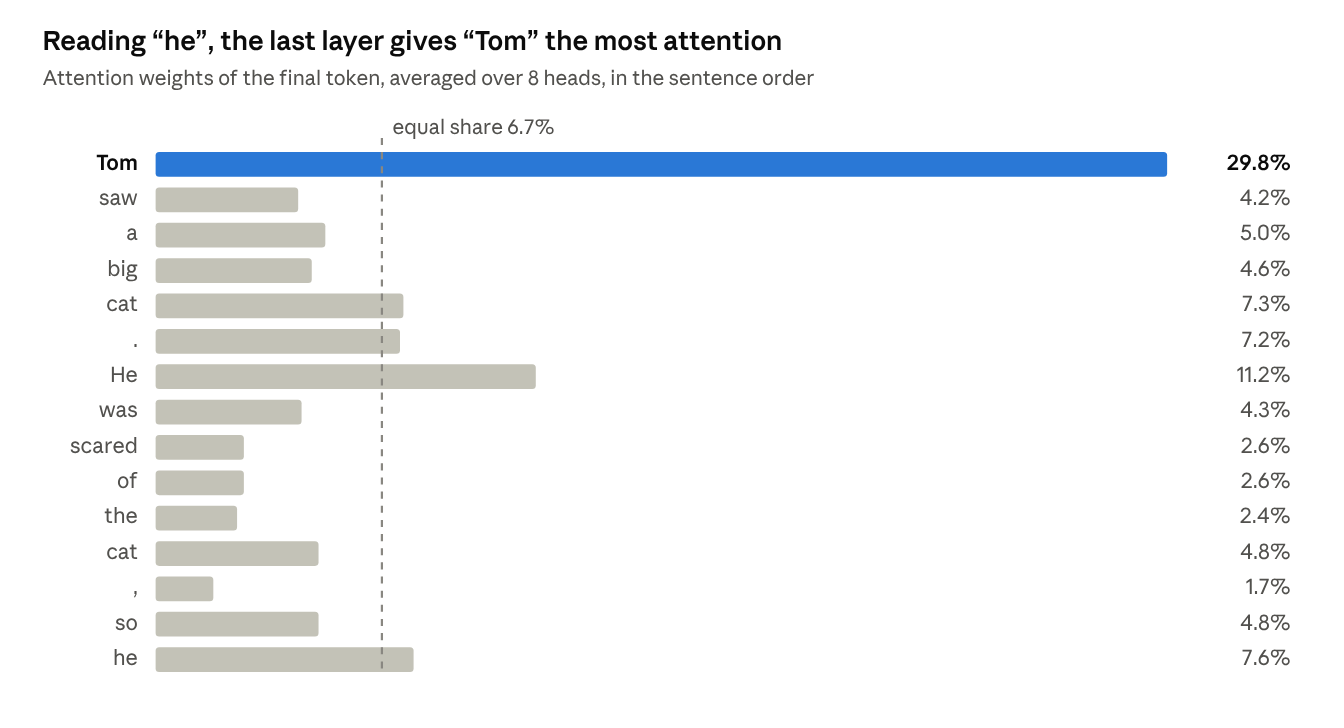
\includegraphics[width=\linewidth]{how-an-llm-works-figures/attention-he.png}
\caption{Measured from the trained 24M model $\cdot$ one sentence, last of 8 layers}
\end{figure}

For this sentence the model predicts \vs{}ran at 48.8\%, \vs{}hid at 8.1\% and \vs{}screamed at 7.8\%. “Tom” gets the largest share, and “He” comes second at 11.2\%.

This was the clearest of three sentences tried, so do not expect it every time. For “Anna and Ben went to the park. Anna found a toy and gave it to”, the model correctly gives \vs{}Ben 91\%, yet its largest last-layer weights fall on “and” and the full stop. Attention weights are a hint and not a full explanation, because each layer works on mixtures made by the layers before it.

\subsection*{What it costs}
\phantomsection
\addcontentsline{toc}{subsection}{What it costs}

Every token scores every earlier token, so the work grows with the square of the context length. At 768 tokens, that is a table of 768 $\times$ 768 = 589,824 scores for each head in each layer. This is the main reason context length has a limit.

\subsection*{What attention alone is missing}
\phantomsection
\addcontentsline{toc}{subsection}{What attention alone is missing}

Attention still has three gaps, and the next sections fill them:

\begin{itemize}
\item It gives each token only one mixture. Section 6 adds several heads.
\item It knows which tokens come earlier, but not how far back they are. Section 7 adds position.
\item Its output is a weighted average of values, which is a weak way to compute. Section 8 adds a non-linear network.
\end{itemize}

\section*{6. Multi-head and grouped-query attention}
\phantomsection
\addcontentsline{toc}{section}{6. Multi-head and grouped-query attention}

One attention pass gives each token one mixture, so the model runs many smaller passes side by side. Grouped-query attention (GQA) then saves parameters by letting those passes share keys and values.

\subsection*{Multi-head attention}
\phantomsection
\addcontentsline{toc}{subsection}{Multi-head attention}

Split the dimension d into h heads of size d/h. Each head has its own Q, K and V and runs attention by itself. The results are joined and passed through one more learned matrix, $W_O$.
\[
\mathrm{MHA}(\mathbf{x}) = \mathbf{W}_O\,[\,\mathrm{head}_1;\ \dots;\ \mathrm{head}_h\,],\qquad \mathrm{head}_m=\mathrm{Attention}(\mathbf{Q}_m,\mathbf{K}_m,\mathbf{V}_m)
\]

Each head is small, so the total work is close to one full-size head. In all three profiles of this repository, each head has 64 dimensions: 384/6, 512/8 and 1,024/16.

Heads learn to look for different things. Back in the “so he” sentence, the 24M model's first layer mostly looks nearby: 5 of its 8 heads put their largest weight on “so”. Its last layer looks far back: 6 of 8 heads put their largest weight on “Tom”. That is one sentence, so take it as an illustration and not a rule.

\subsection*{Grouped-query attention}
\phantomsection
\addcontentsline{toc}{subsection}{Grouped-query attention}

Standard attention gives every query head its own keys and values. GQA keeps all the query heads but uses fewer key and value heads, so several queries read from the same K and V. Think of 16 readers sharing 4 libraries, each asking its own question.

{\small
\begin{longtable}{@{}>{\raggedright\arraybackslash}p{\dimexpr 0.508\linewidth-2\tabcolsep\relax}>{\raggedright\arraybackslash}p{\dimexpr 0.231\linewidth-2\tabcolsep\relax}>{\raggedright\arraybackslash}p{\dimexpr 0.262\linewidth-2\tabcolsep\relax}@{}}
\toprule
\textbf{\code{large} model} & \textbf{Standard} & \textbf{GQA, as used here} \\
\midrule
\endhead
Query heads & 16 & 16 \\
Key and value heads & 16 & 4 \\
Size of k\_proj and v\_proj, each & 1,024 $\times$ 1,024 & 1,024 $\times$ 256 \\
Whole-model parameters & 209,716,224 & 184,550,400 \\
\bottomrule
\end{longtable}
}

That saves 25.2M parameters, about 12\%. The cost is fewer independent kinds of key and value.

Large production models use GQA mainly to shrink the KV cache used when writing text (section 13). This repository has no such cache, so its gain is fewer weights and less work per step.

\begin{figure}[H]
\centering
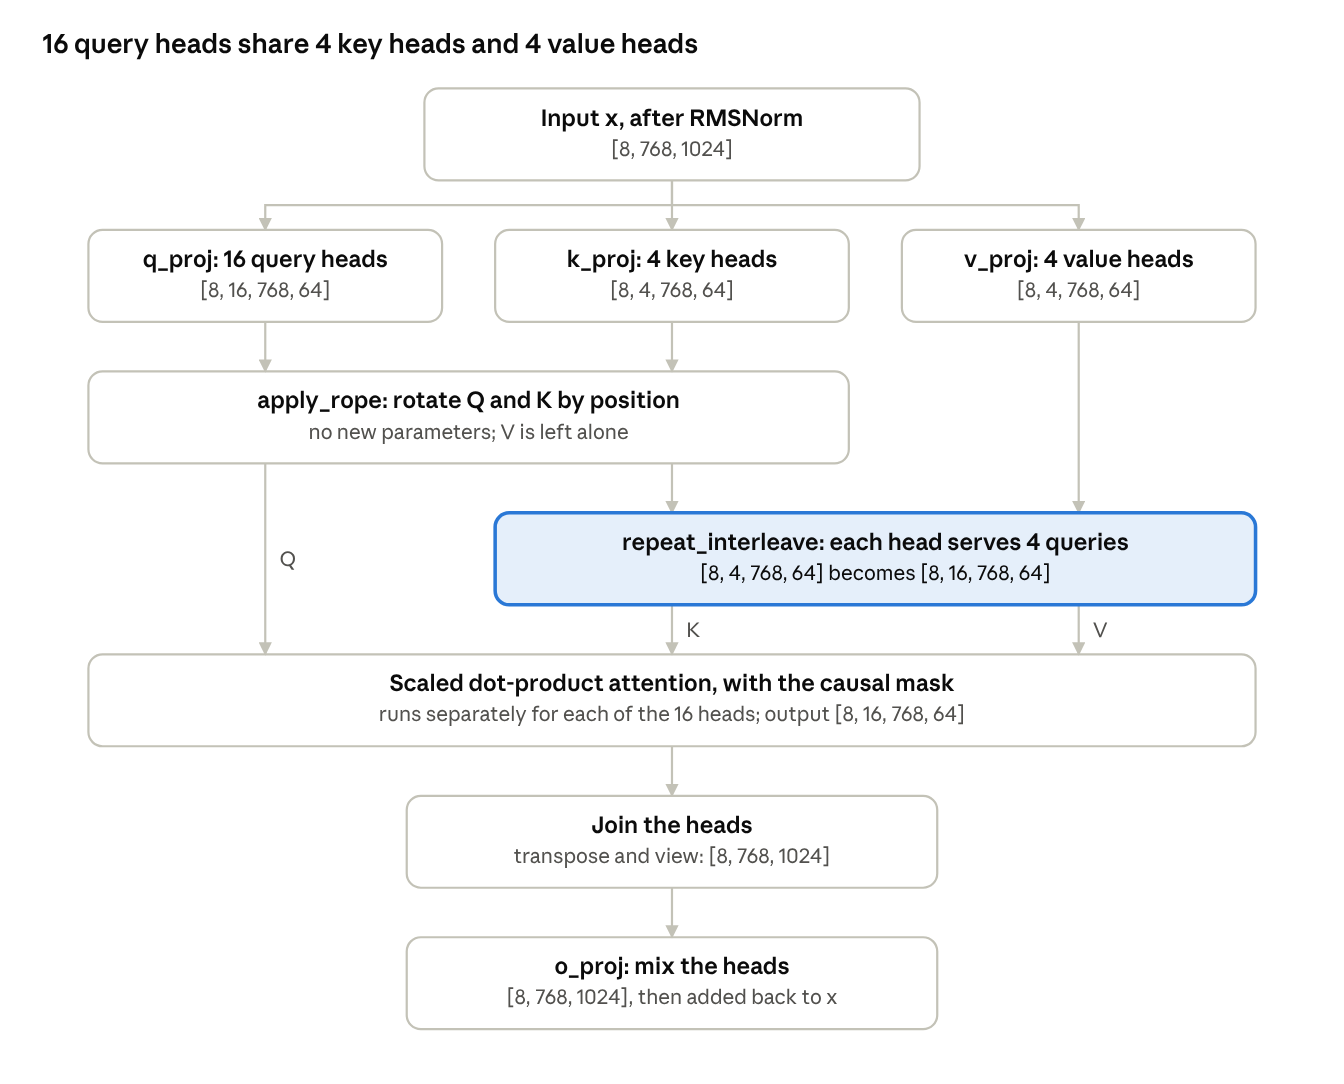
\includegraphics[width=\linewidth]{how-an-llm-works-figures/gqa-flow.png}
\caption{GQAAttention.forward in the large model, with batch 8 and context 768}
\end{figure}

Only the highlighted step makes this different from standard attention. Without it, K and V would simply have 16 heads from the start.

\Needspace{24\baselineskip}
\subsection*{The code}
\phantomsection
\addcontentsline{toc}{subsection}{The code}

\begin{lstlisting}[language=Python]
# model/modern_gpt.py, GQAAttention.forward
B, T, C = x.shape                          # [8, 768, 1024]

q = self.q_proj(x).view(B, T, self.n_heads,    self.head_dim).transpose(1, 2)
k = self.k_proj(x).view(B, T, self.n_kv_heads, self.head_dim).transpose(1, 2)
v = self.v_proj(x).view(B, T, self.n_kv_heads, self.head_dim).transpose(1, 2)

q, k = apply_rope(q, k)                    # section 7

k = k.repeat_interleave(self.repeat, dim=1)
v = v.repeat_interleave(self.repeat, dim=1)

output = F.scaled_dot_product_attention(
    q, k, v,
    dropout_p=self.dropout if self.training else 0.0,
    is_causal=True,
)

output = output.transpose(1, 2).contiguous().view(B, T, C)
return self.o_proj(output)
\end{lstlisting}

\begin{itemize}
\item \textbf{\code{view} then \code{transpose}} cuts the last dimension into heads and moves the head axis forward. PyTorch then treats each head as a separate batch of attention.
\item \textbf{\code{repeat\_\allowbreak{}interleave}} turns heads [k0, k1, k2, k3] into [k0, k0, k0, k0, k1, k1, k1, k1, and so on]. Query heads 0 to 3 read k0, heads 4 to 7 read k1, and so on.
\item \textbf{\code{self.\allowbreak{}repeat}} is \code{n\_\allowbreak{}heads /\allowbreak{}/\allowbreak{} n\_\allowbreak{}kv\_\allowbreak{}heads}, which is 4 here. That is why the constructor raises an error if n\_heads cannot be divided evenly.
\item \textbf{\code{dropout\_\allowbreak{}p}} randomly drops some attention weights during training only, which makes the model rely less on any one connection.
\end{itemize}

\section*{7. Position: how RoPE tells the model word order}
\phantomsection
\addcontentsline{toc}{section}{7. Position: how RoPE tells the model word order}

Attention alone knows which tokens are earlier, but not how far back they are. Rotary position embeddings (RoPE) fix that by rotating Q and K by an angle that grows with position, so each score depends on the distance between two tokens.

\subsection*{Why position needs help}
\phantomsection
\addcontentsline{toc}{subsection}{Why position needs help}

Without position information, the model could not tell a “the” one token back from a “the” 500 tokens back. Yet the difference matters a lot for predicting the next word.

Earlier Transformers added a position vector to each token's embedding. RoPE adds nothing to the embeddings and has no parameters, because it computes everything from the position number.

\subsection*{The math}
\phantomsection
\addcontentsline{toc}{subsection}{The math}

Group the 64 dimensions of a head into 32 pairs. Treat each pair as a 2D point and rotate it with the standard rotation matrix:
\[
\mathbf{R}(\theta)=\begin{bmatrix}\cos\theta&-\sin\theta\\\sin\theta&\cos\theta\end{bmatrix}
\]

The angle depends on the token's position p and on which pair i is being rotated:
\[
\theta_i(p)=\frac{p}{10000^{2i/d}},\qquad i=0,1,\dots,\tfrac{d}{2}-1
\]

Now comes the key step. Take a query pair u rotated by angle $\alpha$, and a key pair w rotated by angle $\beta$. Their dot product is:
\[
\big(\mathbf{R}(\alpha)\mathbf{u}\big)\cdot\big(\mathbf{R}(\beta)\mathbf{w}\big)=\mathbf{u}^{\top}\mathbf{R}(\alpha)^{\top}\mathbf{R}(\beta)\,\mathbf{w}=\mathbf{u}^{\top}\mathbf{R}(\beta-\alpha)\,\mathbf{w}
\]

The result depends only on $\beta$ $-$ $\alpha$. For a query at position m and a key at position n, that difference is (n $-$ m) / $10000^{2i/d}$, so only the gap between the tokens matters. Moving both tokens along by the same amount changes nothing.

\subsection*{Checking it on the real function}
\phantomsection
\addcontentsline{toc}{subsection}{Checking it on the real function}

This test put the same random query vector at every position and the same random key vector at every position, ran the real \code{apply\_\allowbreak{}rope}, and took dot products:

{\small
\begin{longtable}{@{}>{\raggedright\arraybackslash}p{\dimexpr 0.318\linewidth-2\tabcolsep\relax}>{\raggedright\arraybackslash}p{\dimexpr 0.273\linewidth-2\tabcolsep\relax}>{\raggedright\arraybackslash}p{\dimexpr 0.205\linewidth-2\tabcolsep\relax}>{\raggedright\arraybackslash}p{\dimexpr 0.205\linewidth-2\tabcolsep\relax}@{}}
\toprule
\textbf{Query position} & \textbf{Key position} & \textbf{Gap} & \textbf{Score} \\
\midrule
\endhead
10 & 7 & 3 & 3.0397 \\
20 & 17 & 3 & 3.0397 \\
250 & 247 & 3 & 3.0397 \\
10 & 4 & 6 & 6.5890 \\
250 & 244 & 6 & 6.5890 \\
10 & 10 & 0 & 8.5095 \\
250 & 250 & 0 & 8.5095 \\
\bottomrule
\end{longtable}
}

The same gap gives the same score, and a different gap gives a different score. Rotation also keeps a vector's length: 7.5803 before and after in the same test. So RoPE changes direction only, which leaves the scale that section 5 protected unchanged.

\subsection*{Why there are many frequencies}
\phantomsection
\addcontentsline{toc}{subsection}{Why there are many frequencies}

Each pair rotates at its own speed, like the hands of a clock. Fast pairs separate nearby tokens, and slow pairs tell distant tokens apart.

{\small
\begin{longtable}{@{}>{\raggedright\arraybackslash}p{\dimexpr 0.188\linewidth-2\tabcolsep\relax}>{\raggedright\arraybackslash}p{\dimexpr 0.354\linewidth-2\tabcolsep\relax}>{\raggedright\arraybackslash}p{\dimexpr 0.458\linewidth-2\tabcolsep\relax}@{}}
\toprule
\textbf{Pair i} & \textbf{Radians per token} & \textbf{Tokens for a full turn} \\
\midrule
\endhead
0 & 1.0 & 6.3 \\
1 & 0.75 & 8.4 \\
8 & 0.1 & 62.8 \\
16 & 0.01 & 628 \\
31 & 0.00013 & 47,117 \\
\bottomrule
\end{longtable}
}

A single fast hand would repeat every 6 tokens, so a gap of 3 and a gap of 9 could look alike. Together, the 32 speeds make each gap in a 768-token window look different.

\Needspace{18\baselineskip}
\subsection*{The code}
\phantomsection
\addcontentsline{toc}{subsection}{The code}

\begin{lstlisting}[language=Python]
# model/modern_gpt.py
def rotate_half(x):
    half = x.shape[-1] // 2
    return torch.cat([-x[..., half:], x[..., :half]], dim=-1)

def apply_rope(q, k):
    seq_len, head_dim, device = q.shape[-2], q.shape[-1], q.device
    inv_freq = 1.0 / (10000 ** (torch.arange(0, head_dim, 2, device=device, dtype=torch.float32) / head_dim))
    positions = torch.arange(seq_len, device=device, dtype=torch.float32)
    freqs = torch.outer(positions, inv_freq)     # one angle per position and pair
    emb = torch.cat([freqs, freqs], dim=-1)
    cos, sin = emb.cos()[None, None, :, :], emb.sin()[None, None, :, :]
    return q * cos + rotate_half(q) * sin, k * cos + rotate_half(k) * sin
\end{lstlisting}

The last line is the rotation matrix written out. Dimension j pairs with dimension j + 32. Call the two values a and b, and the matrix gives:
\[
a' = a\cos\theta - b\sin\theta,\qquad b' = b\cos\theta + a\sin\theta
\]

\code{rotate\_\allowbreak{}half} builds [$-$b, a], and \code{x * cos + rotate\_\allowbreak{}half(x) * sin} then gives exactly those two lines.

\subsection*{Three details worth noticing}
\phantomsection
\addcontentsline{toc}{subsection}{Three details worth noticing}

\begin{itemize}
\item \textbf{V is not rotated.} Position should change which tokens get looked at, not what they hand over.
\item \textbf{K is rotated before it is repeated.} Query heads that share a key head all see the same rotated keys.
\item \textbf{Sliding context is safe.} When writing past 768 tokens, the window slides and positions restart from 0. Only gaps matter, so the scores stay valid.
\end{itemize}

\section*{8. The transformer block}
\phantomsection
\addcontentsline{toc}{section}{8. The transformer block}

A block does two jobs in order: attention lets tokens communicate, then SwiGLU lets each token process what it received. RMSNorm and residual connections keep a deep stack of these blocks trainable.

\Needspace{6\baselineskip}
\begin{lstlisting}[language=Python]
# model/modern_gpt.py, TransformerBlock.forward
x = x + self.attention(self.norm1(x))
x = x + self.ffn(self.norm2(x))
return x
\end{lstlisting}

\begin{figure}[H]
\centering
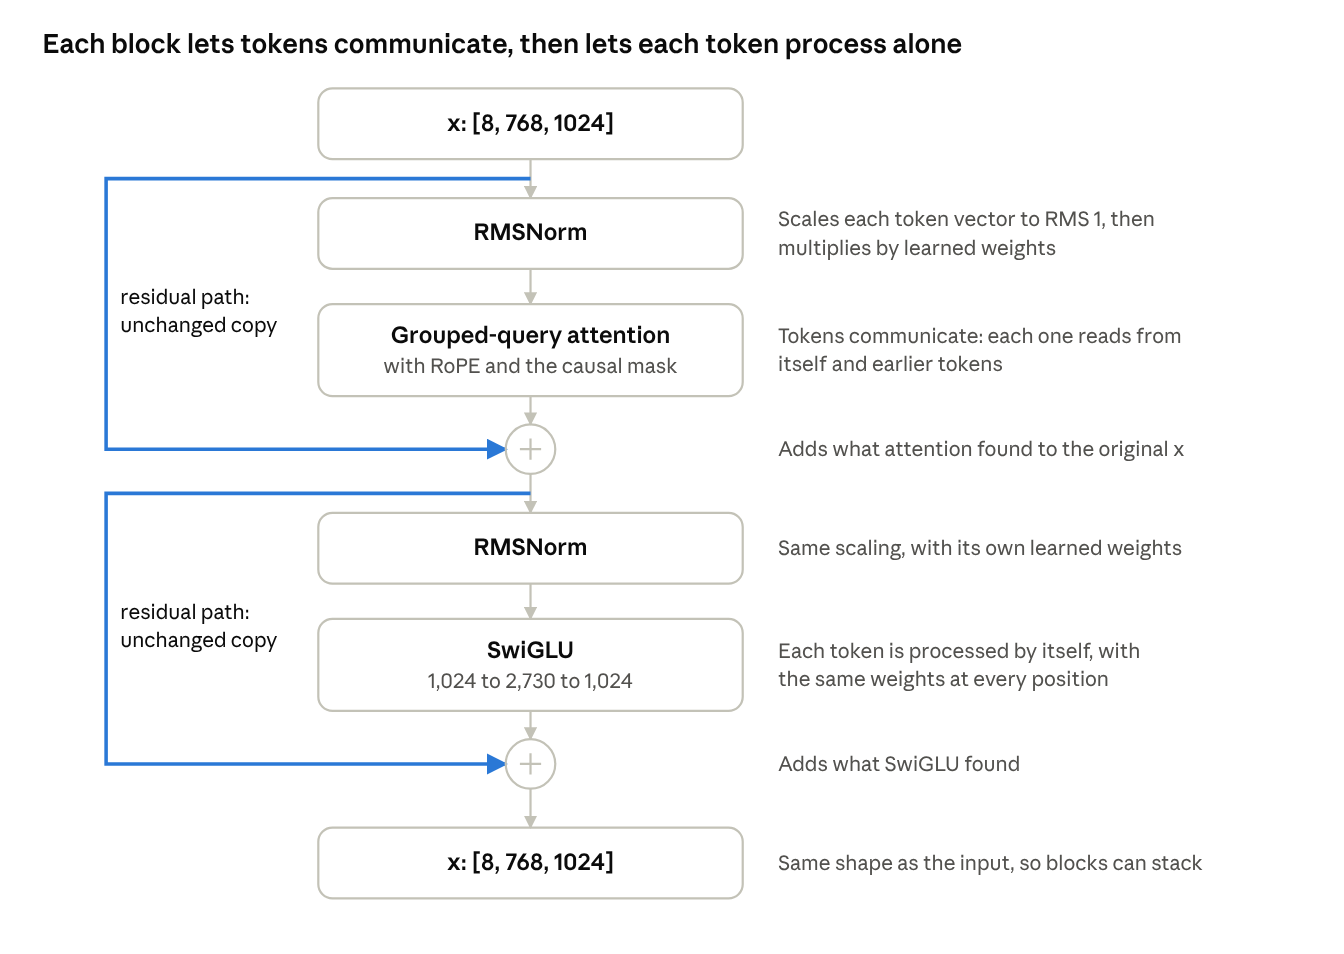
\includegraphics[width=\linewidth]{how-an-llm-works-figures/transformer-block.png}
\caption{TransformerBlock.forward in the large model}
\end{figure}

\subsection*{RMSNorm: keep vectors at a steady size}
\phantomsection
\addcontentsline{toc}{subsection}{RMSNorm: keep vectors at a steady size}

Numbers can drift larger or smaller as they pass through many layers, and that makes gradients unstable. RMSNorm rescales each token's vector so that its root mean square is 1, then multiplies by learned weights w.
\[
\mathrm{RMS}(\mathbf{x})=\sqrt{\frac{1}{d}\sum_{i=1}^{d}x_i^2},\qquad
\mathrm{RMSNorm}(\mathbf{x})=\mathbf{w}\odot\frac{\mathbf{x}}{\sqrt{\mathrm{RMS}(\mathbf{x})^2+\epsilon}}
\]

\Needspace{6\baselineskip}
\begin{lstlisting}[language=Python]
# model/modern_gpt.py, RMSNorm.forward
variance = x.float().pow(2).mean(dim=-1, keepdim=True)
x = x * torch.rsqrt(variance + self.eps)
return self.weight * x
\end{lstlisting}

With w still at its starting value of 1, the real class turns [3, 4] into [0.849, 1.131], and its RMS is 1. It turns [30, 40] into the same result, so only the vector's direction survives.

The older LayerNorm also subtracts the mean, and RMSNorm skips that step. The variance is computed in 32-bit floats because squares overflow easily in the 16-bit floats used during training.

\subsection*{Residual connections: a clean path for gradients}
\phantomsection
\addcontentsline{toc}{subsection}{Residual connections: a clean path for gradients}

Each block adds its result to its input and does not replace it. Take the derivative of the output with respect to the input:
\[
\mathbf{x}_{\text{out}} = \mathbf{x} + f(\mathbf{x}),\qquad
\frac{\partial \mathbf{x}_{\text{out}}}{\partial \mathbf{x}} = \mathbf{I} + \frac{\partial f(\mathbf{x})}{\partial \mathbf{x}}
\]

Backpropagation multiplies one such factor per block. Without the identity matrix I, a long product of matrices can shrink toward zero or blow up. With it, the gradient always has a direct route back to the first layers.

There is a second benefit. Each block only needs to learn a correction to x, and a block that has learned nothing yet still passes x through.

This repository uses pre-normalization: RMSNorm is applied to the input of each sub-layer, so the residual path itself is never rescaled. That is why the model needs one final \code{self.\allowbreak{}norm} before the output layer.

\subsection*{SwiGLU: the computing step}
\phantomsection
\addcontentsline{toc}{subsection}{SwiGLU: the computing step}

Attention's output is a weighted average of values, so the model needs a separate non-linear step. SwiGLU applies one to each token.
\[
\mathrm{SiLU}(z)=z\,\sigma(z),\qquad
\mathrm{SwiGLU}(\mathbf{x})=\mathbf{W}_{\text{down}}\big(\mathrm{SiLU}(\mathbf{W}_{\text{gate}}\mathbf{x})\odot\mathbf{W}_{\text{up}}\mathbf{x}\big)
\]

\Needspace{5\baselineskip}
\begin{lstlisting}[language=Python]
# model/modern_gpt.py, SwiGLU.forward
x = F.silu(self.gate(x)) * self.up(x)
return self.dropout(self.down(x))
\end{lstlisting}

The element-wise product is the “gate”: one learned signal controls how much of another signal passes through. A plain network with one activation function has no such multiplication between two learned signals.

The linear layers act only on the last dimension, so every position uses the same weights and no information crosses between tokens here. All communication happens in attention.

The hidden size is about 8/3 of d, which is why 1,024 becomes 2,730. A classic feed-forward layer has 2 matrices of d $\times$ 4d, or 8d\textsuperscript{2} weights. SwiGLU has 3 matrices of d $\times$ (8/3)d, which is also 8d\textsuperscript{2}, so it costs about the same.

This is where most of the weights are. In the \code{large} model, SwiGLU holds 8,386,560 of the 11,010,048 weights in each block, which is 76\%.

\subsection*{Dropout}
\phantomsection
\addcontentsline{toc}{subsection}{Dropout}

With \code{dropout = 0.\allowbreak{}1}, training randomly zeroes 10\% of SwiGLU's outputs and of the attention weights. The model cannot rely on any single connection, which reduces memorizing. \code{model.\allowbreak{}eval()} turns dropout off for scoring and writing.

\subsection*{Why stack many blocks}
\phantomsection
\addcontentsline{toc}{subsection}{Why stack many blocks}

One block lets a token read earlier tokens. The next block reads vectors that already contain those mixtures, so facts can pass from token to token across layers and combine. The \code{large} model stacks 16 blocks, and all of them share the same shape, so stacking more only needs a bigger \code{n\_\allowbreak{}layers}.

\section*{9. The whole model}
\phantomsection
\addcontentsline{toc}{section}{9. The whole model}

The model is an embedding, a stack of blocks, one last RMSNorm and a linear output layer. Tensors keep the shape [B, T, d] all the way through, until the output layer turns d into the vocabulary size.

\Needspace{16\baselineskip}
\begin{lstlisting}[language=Python]
# model/modern_gpt.py, ModernGPT.forward (checkpointing option left out)
def forward(self, idx, targets=None):
    B, T = idx.shape
    if T > self.block_size:
        raise ValueError("Sequence exceeds context length.")

    x = self.embedding(idx)
    for block in self.blocks:
        x = block(x)
    x = self.norm(x)
    logits = self.lm_head(x)

    loss = None
    if targets is not None:
        loss = F.cross_entropy(logits.reshape(-1, logits.size(-1)), targets.reshape(-1))
    return logits, loss
\end{lstlisting}

\subsection*{Every tensor shape}
\phantomsection
\addcontentsline{toc}{subsection}{Every tensor shape}

These shapes come from the real \code{large} model, with 8 windows of 768 tokens. B is the batch, T is the context, and d is the model dimension.

{\small
\begin{longtable}{@{}>{\raggedright\arraybackslash}p{\dimexpr 0.315\linewidth-2\tabcolsep\relax}>{\raggedright\arraybackslash}p{\dimexpr 0.478\linewidth-2\tabcolsep\relax}>{\raggedright\arraybackslash}p{\dimexpr 0.207\linewidth-2\tabcolsep\relax}@{}}
\toprule
\textbf{Stage} & \textbf{Code} & \textbf{Shape} \\
\midrule
\endhead
Token ids & idx & [8, 768] \\
After embedding & self.embedding(idx) & [8, 768, 1024] \\
Queries & q\_proj, view, transpose & [8, 16, 768, 64] \\
Keys and values & k\_proj, v\_proj, view, transpose & [8, 4, 768, 64] \\
After repeating & repeat\_interleave & [8, 16, 768, 64] \\
Score table, inside attention & Q times K transposed & [8, 16, 768, 768] \\
Attention output & scaled\_dot\_product\_attention & [8, 16, 768, 64] \\
Heads joined & transpose, view, o\_proj & [8, 768, 1024] \\
Inside SwiGLU & gate, up & [8, 768, 2730] \\
After one block & down, then residual & [8, 768, 1024] \\
After 16 blocks and norm & self.norm(x) & [8, 768, 1024] \\
Scores for every token & self.lm\_head(x) & [8, 768, 8192] \\
\bottomrule
\end{longtable}
}

The last shape says it all: for each of 8 windows and 768 positions, there are 8,192 scores for the next token. These raw scores are called logits.

\subsection*{Weight tying: one matrix used twice}
\phantomsection
\addcontentsline{toc}{subsection}{Weight tying: one matrix used twice}

The output layer shares its weights with the embedding, through one line of code:

\Needspace{3\baselineskip}
\begin{lstlisting}[language=Python]
self.lm_head.weight = self.embedding.weight
\end{lstlisting}

That makes the score of token j the dot product of the final vector h with token j's embedding:
\[
z_j = \mathbf{h}\cdot\mathbf{e}_j
\]

So the model's output is a vector meaning “the next token should look like this”. Tokens whose embeddings point the same way get high scores. This fits section 4: \vs{}girl, \vs{}boy and \vs{}dog have nearby embeddings, and they get high probability together.

Computing h $\cdot$ E by hand on the trained 24M model gave the same values as the model's logits. Tying also saves 8,388,608 parameters in the \code{large} model.

\subsection*{Counting every parameter}
\phantomsection
\addcontentsline{toc}{subsection}{Counting every parameter}

A linear layer without bias has input size $\times$ output size weights, and this model uses no bias anywhere. Multiplying it out for \code{large} matches the 184,550,400 that training prints:

{\small
\begin{longtable}{@{}>{\raggedright\arraybackslash}p{\dimexpr 0.456\linewidth-2\tabcolsep\relax}>{\raggedright\arraybackslash}p{\dimexpr 0.191\linewidth-2\tabcolsep\relax}>{\raggedright\arraybackslash}p{\dimexpr 0.132\linewidth-2\tabcolsep\relax}>{\raggedright\arraybackslash}p{\dimexpr 0.221\linewidth-2\tabcolsep\relax}@{}}
\toprule
\textbf{Part} & \textbf{One copy} & \textbf{Copies} & \textbf{Total} \\
\midrule
\endhead
Embedding, shared with lm\_head & 8,192 $\times$ 1,024 & 1 & 8,388,608 \\
q\_proj & 1,024 $\times$ 1,024 & 16 & 16,777,216 \\
k\_proj & 1,024 $\times$ 256 & 16 & 4,194,304 \\
v\_proj & 1,024 $\times$ 256 & 16 & 4,194,304 \\
o\_proj & 1,024 $\times$ 1,024 & 16 & 16,777,216 \\
gate & 1,024 $\times$ 2,730 & 16 & 44,728,320 \\
up & 1,024 $\times$ 2,730 & 16 & 44,728,320 \\
down & 2,730 $\times$ 1,024 & 16 & 44,728,320 \\
norm1 and norm2 & 1,024 each & 32 & 32,768 \\
Final norm & 1,024 & 1 & 1,024 \\
Total &  &  & 184,550,400 \\
\bottomrule
\end{longtable}
}

RoPE, masks and softmax add nothing, because they have no weights.

\subsection*{The model sizes in this repository}
\phantomsection
\addcontentsline{toc}{subsection}{The model sizes in this repository}

These profiles live in \code{training/\allowbreak{}config.\allowbreak{}py}. All use a context of 768 tokens and a head size of 64, and vocabulary size comes from the tokenizer.

{\small
\begin{longtable}{@{}>{\raggedright\arraybackslash}p{\dimexpr 0.128\linewidth-2\tabcolsep\relax}>{\raggedright\arraybackslash}p{\dimexpr 0.105\linewidth-2\tabcolsep\relax}>{\raggedright\arraybackslash}p{\dimexpr 0.105\linewidth-2\tabcolsep\relax}>{\raggedright\arraybackslash}p{\dimexpr 0.198\linewidth-2\tabcolsep\relax}>{\raggedright\arraybackslash}p{\dimexpr 0.128\linewidth-2\tabcolsep\relax}>{\raggedright\arraybackslash}p{\dimexpr 0.163\linewidth-2\tabcolsep\relax}>{\raggedright\arraybackslash}p{\dimexpr 0.174\linewidth-2\tabcolsep\relax}@{}}
\toprule
\textbf{Profile} & \textbf{d} & \textbf{Layers} & \textbf{Query / key heads} & \textbf{SwiGLU size} & \textbf{Vocabulary} & \textbf{Parameters} \\
\midrule
\endhead
\code{small} & 384 & 6 & 6 / 2 & 1,024 & 4,096 & 11,015,040 \\
\code{medium} & 512 & 8 & 8 / 2 & 1,365 & 4,096 & 24,121,856 \\
\code{large} & 1,024 & 16 & 16 / 4 & 2,730 & 8,192 & 184,550,400 \\
\bottomrule
\end{longtable}
}

\subsection*{Why a checkpoint is 12 bytes per parameter}
\phantomsection
\addcontentsline{toc}{subsection}{Why a checkpoint is 12 bytes per parameter}

Each weight takes 4 bytes. AdamW keeps two more numbers for each weight, as section 11 shows, which adds 8 bytes. So the \code{large} checkpoint should be 184,550,400 $\times$ 12 = 2.21 GB, and the real file is 2,214,798,763 bytes.

\section*{10. Loss: measuring surprise}
\phantomsection
\addcontentsline{toc}{section}{10. Loss: measuring surprise}

Loss is the model's average surprise at the real next token. A certain, correct guess costs 0, and a token given 1\% probability costs 4.6. Training does nothing except push this one number down.

\subsection*{From scores to probabilities}
\phantomsection
\addcontentsline{toc}{subsection}{From scores to probabilities}

Softmax turns the logits z into probabilities that are positive and add up to 1:
\[
p_j = \frac{\exp(z_j)}{\sum_{l=1}^{V}\exp(z_l)}
\]

\subsection*{Cross-entropy}
\phantomsection
\addcontentsline{toc}{subsection}{Cross-entropy}

For each position t, take the probability the model gave to the real next token $y_t$. The loss is the average of its negative log over all N positions:
\[
\mathcal{L} = -\frac{1}{N}\sum_{t=1}^{N}\ln p_t(y_t)
\]

The log has a clear reason. The probability of a whole text is the product of its next-token probabilities, and the log turns that product into a sum. So lowering this loss makes the training text as probable as possible under the model, which is called maximum likelihood.

The log also punishes confident mistakes hard. A probability of 0.01 costs 4.6, and a probability of 0.000001 costs 13.8.

\Needspace{4\baselineskip}
\begin{lstlisting}[language=Python]
# model/modern_gpt.py, ModernGPT.forward
loss = F.cross_entropy(logits.reshape(-1, logits.size(-1)), targets.reshape(-1))
\end{lstlisting}

The \code{reshape} flattens [8, 768, 8192] into [6144, 8192], and the targets into [6144], because the function expects one row per prediction. It applies log-softmax itself, so the model's forward pass has no softmax.

\subsection*{Real numbers from the trained model}
\phantomsection
\addcontentsline{toc}{subsection}{Real numbers from the trained model}

Here is the trained 24M model reading an ordinary story opening. Each row shows the last token it has read, the real next token, and what it thought of that token.

{\small
\begin{longtable}{@{}>{\raggedright\arraybackslash}p{\dimexpr 0.246\linewidth-2\tabcolsep\relax}>{\raggedright\arraybackslash}p{\dimexpr 0.246\linewidth-2\tabcolsep\relax}>{\raggedright\arraybackslash}p{\dimexpr 0.246\linewidth-2\tabcolsep\relax}>{\raggedright\arraybackslash}p{\dimexpr 0.262\linewidth-2\tabcolsep\relax}@{}}
\toprule
\textbf{Last token read} & \textbf{Real next token} & \textbf{Probability} & \textbf{Surprise ($-$ln p)} \\
\midrule
\endhead
Once & \vs{}upon & 94.4\% & 0.058 \\
\vs{}upon & \vs{}a & 99.99\% & 0.000 \\
\vs{}a & \vs{}time & 99.99\% & 0.000 \\
\vs{}time & comma & 93.3\% & 0.070 \\
comma & \vs{}there & 80.6\% & 0.216 \\
\vs{}there & \vs{}was & 97.5\% & 0.025 \\
\vs{}was & \vs{}a & 98.3\% & 0.017 \\
\vs{}a & \vs{}little & 43.4\% & 0.835 \\
\vs{}little & \vs{}girl & 45.1\% & 0.797 \\
\vs{}girl & \vs{}named & 92.4\% & 0.079 \\
\vs{}named & \vs{}Lily & 35.3\% & 1.042 \\
\vs{}Lily & full stop & 99.5\% & 0.005 \\
\bottomrule
\end{longtable}
}

The mean is the loss for this sentence: 0.262. The fixed phrase costs almost nothing, and the real choices (little, girl, Lily) cost the most.

Now change the ending to something the stories never contain, “a little quantum computer”:

{\small
\begin{longtable}{@{}>{\raggedright\arraybackslash}p{\dimexpr 0.246\linewidth-2\tabcolsep\relax}>{\raggedright\arraybackslash}p{\dimexpr 0.246\linewidth-2\tabcolsep\relax}>{\raggedright\arraybackslash}p{\dimexpr 0.246\linewidth-2\tabcolsep\relax}>{\raggedright\arraybackslash}p{\dimexpr 0.262\linewidth-2\tabcolsep\relax}@{}}
\toprule
\textbf{Last token read} & \textbf{Real next token} & \textbf{Probability} & \textbf{Surprise ($-$ln p)} \\
\midrule
\endhead
\vs{}little & \vs{}qu & 0.0003\% & 12.78 \\
\vs{}qu & ant & 0.003\% & 10.40 \\
ant & um & 0.02\% & 8.44 \\
um & \vs{}computer & 0.004\% & 10.11 \\
\vs{}computer & full stop & 85.9\% & 0.15 \\
\bottomrule
\end{longtable}
}

The mean for this whole sentence jumps to 3.315. Notice the last row: even after a strange sentence, the model expects a full stop after “computer”.

\subsection*{The starting point: ln V}
\phantomsection
\addcontentsline{toc}{subsection}{The starting point: ln V}

An untrained model has no preference, so it gives each token about 1/V, and the loss starts near ln V:
\[
\mathcal{L}_0 = -\ln\frac{1}{V} = \ln V
\]

For V = 8,192, that is 9.01. The real untrained 185M model scored 9.26, a little higher because its random logits are not all equal. This is a useful check: if a new model starts far from ln V, look for a bug before training.

\subsection*{Perplexity: the same number, easier to picture}
\phantomsection
\addcontentsline{toc}{subsection}{Perplexity: the same number, easier to picture}

Perplexity is e raised to the loss. Think of it as the number of equally likely tokens the model is effectively choosing between.
\[
\mathrm{perplexity} = e^{\mathcal{L}}
\]

These all use the same data and tokenizer, so they compare directly:

{\small
\begin{longtable}{@{}>{\raggedright\arraybackslash}p{\dimexpr 0.561\linewidth-2\tabcolsep\relax}>{\raggedright\arraybackslash}p{\dimexpr 0.227\linewidth-2\tabcolsep\relax}>{\raggedright\arraybackslash}p{\dimexpr 0.212\linewidth-2\tabcolsep\relax}@{}}
\toprule
\textbf{Predictor on TinyStories} & \textbf{Validation loss} & \textbf{Perplexity} \\
\midrule
\endhead
Uniform guess over 4,096 tokens & 8.318 & 4,096 \\
Bigram table, sees one previous token & 3.982 & 53.6 \\
\code{small} model, 11.0M parameters & 1.282 & 3.6 \\
\code{medium} model, 24.1M parameters & 1.110 & 3.0 \\
\bottomrule
\end{longtable}
}

\subsection*{Bits per character: comparing different tokenizers}
\phantomsection
\addcontentsline{toc}{subsection}{Bits per character: comparing different tokenizers}

Loss per token cannot compare two tokenizers, because a bigger token is harder to predict but covers more text. Dividing by characters per token fixes that:
\[
\text{bits per character} = \frac{\mathcal{L}}{\ln 2 \times \text{characters per token}}
\]

The \code{medium} model has a loss of 1.110 and 3.93 characters per token, which gives about 0.41 bits per character. A plain ASCII character takes 8 bits, so this model could compress these stories about 20 times. Prediction and compression are the same problem: a model that guesses well needs few bits to pin down what actually came next.

\subsection*{What loss does not tell you}
\phantomsection
\addcontentsline{toc}{subsection}{What loss does not tell you}

Low loss means the text looks like the training data. It does not mean the text is true, because loss has no notion of truth. Section 14 returns to this.

\section*{11. Training: how the weights get better}
\phantomsection
\addcontentsline{toc}{section}{11. Training: how the weights get better}

Training repeats one loop: sample windows, compute the loss, compute the gradients, and move every weight a little in the direction that lowers the loss. Everything else in this section makes that loop stable or makes it fit in memory.

\Needspace{22\baselineskip}
\subsection*{The loop}
\phantomsection
\addcontentsline{toc}{subsection}{The loop}

\begin{lstlisting}[language=Python]
# training/train.py, main (update mode and logging left out)
for step in range(start, start + steps):
    current_lr = lr(step, run["total_steps"], run["peak_lr"])
    for g in opt.param_groups:
        g["lr"] = current_lr

    for micro in range(config.gradient_accumulation_steps):
        x, y = batch(train, cfg["block_size"], config.batch_size, device)
        with amp(device):
            _, loss = model(x, y)
            loss = loss / config.gradient_accumulation_steps
        scaler.scale(loss).backward()

    scaler.unscale_(opt)
    torch.nn.utils.clip_grad_norm_(model.parameters(), config.grad_clip)
    scaler.step(opt)
    scaler.update()
    opt.zero_grad(set_to_none=True)
\end{lstlisting}

\subsection*{Backpropagation}
\phantomsection
\addcontentsline{toc}{subsection}{Backpropagation}

The gradient of a weight says how much the loss would change if that weight changed a little. \code{backward()} applies the chain rule from the loss back through every layer, and finds all 184.55M gradients in one pass.

The simplest update is plain gradient descent, where $\eta$ is the learning rate:
\[
\boldsymbol{\theta} \leftarrow \boldsymbol{\theta} - \eta\,\mathbf{g}
\]

\subsection*{AdamW: a better update rule}
\phantomsection
\addcontentsline{toc}{subsection}{AdamW: a better update rule}

Plain gradient descent has two problems. Each batch gives a noisy gradient, and different weights need very different step sizes. AdamW keeps two running averages for each weight to deal with this:
\[
\begin{aligned}
\mathbf{m}_t &= \beta_1\mathbf{m}_{t-1}+(1-\beta_1)\mathbf{g}_t\\
\mathbf{v}_t &= \beta_2\mathbf{v}_{t-1}+(1-\beta_2)\mathbf{g}_t^2\\
\hat{\mathbf{m}}_t &= \mathbf{m}_t/(1-\beta_1^t),\qquad \hat{\mathbf{v}}_t = \mathbf{v}_t/(1-\beta_2^t)\\
\boldsymbol{\theta}' &= \boldsymbol{\theta}_{t-1}-\eta\lambda\,\boldsymbol{\theta}_{t-1}\\
\boldsymbol{\theta}_t &= \boldsymbol{\theta}'-\eta\,\hat{\mathbf{m}}_t\big/\big(\sqrt{\hat{\mathbf{v}}_t}+\epsilon\big)
\end{aligned}
\]

{\small
\begin{longtable}{@{}>{\raggedright\arraybackslash}p{\dimexpr 0.094\linewidth-2\tabcolsep\relax}>{\raggedright\arraybackslash}p{\dimexpr 0.646\linewidth-2\tabcolsep\relax}>{\raggedright\arraybackslash}p{\dimexpr 0.260\linewidth-2\tabcolsep\relax}@{}}
\toprule
\textbf{Line} & \textbf{What it does} & \textbf{Value here} \\
\midrule
\endhead
m & Running mean of the gradient (momentum), which smooths out noise & $\beta_1$ = 0.9 \\
v & Running mean of the squared gradient, which measures each weight's scale & $\beta_2$ = 0.95 \\
$\hat{m}$, $\hat{v}$ & Correct for both averages starting at zero &  \\
$\theta'$ & Weight decay: shrinks every weight a little toward 0 & $\lambda$ = 0.1 \\
$\theta$ & The step: dividing by $\sqrt{\hat{v}}$ gives each weight its own step size & $\eta$ from the schedule below \\
\bottomrule
\end{longtable}
}

The W in AdamW means weight decay is applied directly to the weight, separately from the gradient. Decay discourages large weights, which is another guard against memorizing.

\code{make\_\allowbreak{}optimizer} leaves two kinds of weight out of decay. RMSNorm's scale vectors are not patterns to shrink, and the embedding is the shared matrix from section 9.

\Needspace{5\baselineskip}
\begin{lstlisting}[language=Python]
# training/train.py, make_optimizer
for p in model.parameters():
    (no_decay if p.ndim < 2 or p is embedding else decay).append(p)
\end{lstlisting}

The values m and v are the 8 extra bytes per weight from section 9. They must be saved in the checkpoint, or a resumed run would lose its optimizer's memory.

\subsection*{Learning-rate schedule}
\phantomsection
\addcontentsline{toc}{subsection}{Learning-rate schedule}

The learning rate rises in a straight line during warmup, then follows a cosine curve down to a floor. The formula uses step s, warmup length $S_w$, total steps S and floor ratio r:
\[
\eta(s)=\begin{cases}
\eta_{\text{peak}}\,\dfrac{s+1}{S_w} & s<S_w\\[6pt]
\eta_{\text{peak}}\big(r+(1-r)\,\tfrac12(1+\cos\pi p)\big) & s\ge S_w
\end{cases},\qquad p=\frac{s-S_w}{S-S_w}
\]

\Needspace{8\baselineskip}
\begin{lstlisting}[language=Python]
# training/train.py
def lr(step, total, peak):
    if step < config.warmup_steps:
        return peak * max(1, step + 1) / config.warmup_steps
    p = min(1.0, (step - config.warmup_steps) / max(1, total - config.warmup_steps))
    c = 0.5 * (1 + math.cos(math.pi * p))
    return peak * (config.min_lr_ratio + (1 - config.min_lr_ratio) * c)
\end{lstlisting}

\begin{figure}[H]
\centering
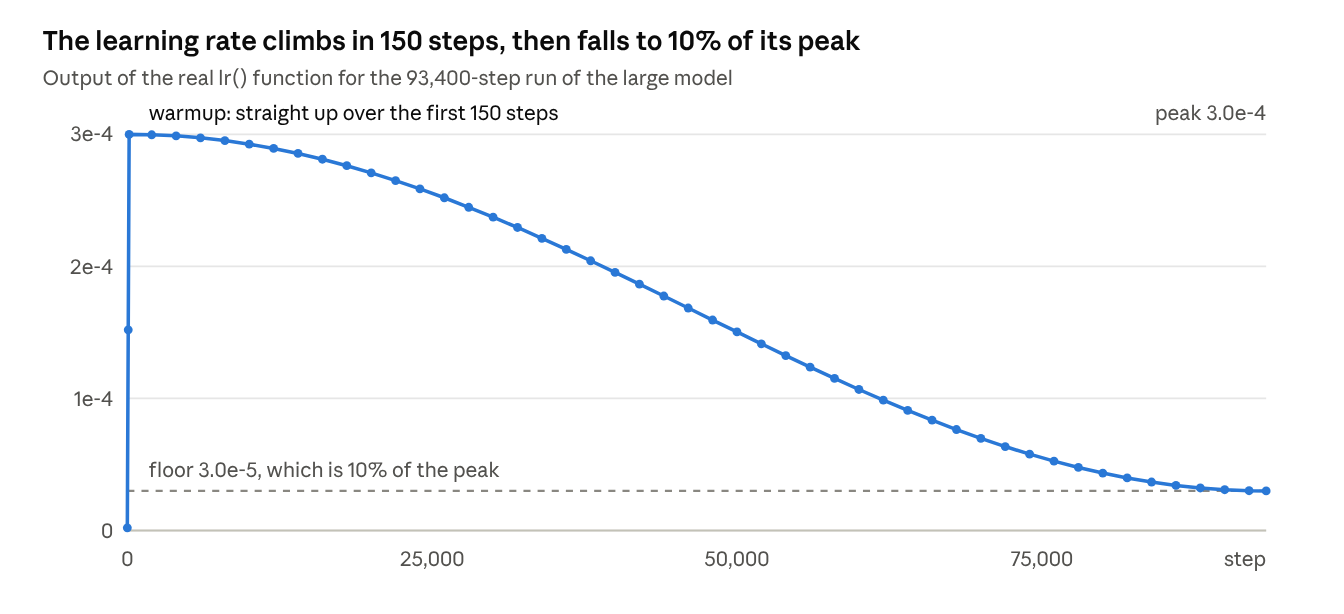
\includegraphics[width=\linewidth]{how-an-llm-works-figures/lr-schedule.png}
\caption{Computed by lr() in training/train.py $\cdot$ peak 3e-4, warmup 150, total 93,400 steps}
\end{figure}

Warmup exists because the first gradients are the least reliable: the weights are random, and Adam's averages hold almost nothing yet. Later, big steps cover ground quickly but keep bouncing around a good solution, so the rate falls to let the weights settle.

You can check the formula against a real run. At step 7,999 it gives 2.95e-4, and the training log printed \code{lr 2.\allowbreak{}95e-04} at that step.

\subsection*{Gradient clipping}
\phantomsection
\addcontentsline{toc}{subsection}{Gradient clipping}

A rare batch can produce a huge gradient and undo hours of work. Clipping limits the combined size of all the gradients to c, which is 1.0 here, and keeps their direction.
\[
\mathbf{g}\leftarrow\mathbf{g}\cdot\min\!\left(1,\frac{c}{\lVert\mathbf{g}\rVert}\right)
\]

\subsection*{Gradient accumulation: a big batch in small memory}
\phantomsection
\addcontentsline{toc}{subsection}{Gradient accumulation: a big batch in small memory}

A bigger batch gives a smoother gradient, but GPU memory limits how many windows fit at once. So the code runs 4 forward and backward passes of 8 windows, then takes one step.

The math works because the gradient of an average is the average of the gradients. Dividing each loss by 4 gives the same gradient as one batch of 32 windows, while memory holds only 8 at a time.
\[
\mathbf{g}=\nabla\Big(\tfrac14\sum_{k=1}^{4}\mathcal{L}_k\Big)=\tfrac14\sum_{k=1}^{4}\nabla\mathcal{L}_k
\]

PyTorch adds each \code{backward()} result to the stored gradients. That is why \code{zero\_\allowbreak{}grad} runs only after the step, and not before each pass.

\subsection*{Mixed precision: faster and smaller}
\phantomsection
\addcontentsline{toc}{subsection}{Mixed precision: faster and smaller}

Inside \code{autocast}, most math runs in 16-bit floats, which saves memory and time, while the weights themselves stay 32-bit. The risk is that 16-bit floats cannot hold very small numbers, so tiny gradients would round to 0.

\code{GradScaler} solves this in four moves:

\begin{enumerate}
\item \code{scaler.\allowbreak{}scale(loss).\allowbreak{}backward()} multiplies the loss by a large factor, so the gradients are large enough to survive.
\item \code{scaler.\allowbreak{}unscale\_\allowbreak{}(opt)} divides them back, so clipping sees their true size.
\item \code{scaler.\allowbreak{}step(opt)} applies the update, but skips it if any gradient is infinite or not a number.
\item \code{scaler.\allowbreak{}update()} lowers the factor after a skipped step and slowly raises it otherwise.
\end{enumerate}

\subsection*{Saving and resuming}
\phantomsection
\addcontentsline{toc}{subsection}{Saving and resuming}

Every check saves the weights, m and v, the step number and the random-number state. The file is written to a temporary name and then renamed, so a power cut cannot leave a half-written checkpoint. \code{--mode resume} then continues on the same schedule.

\section*{12. Reading the results}
\phantomsection
\addcontentsline{toc}{section}{12. Reading the results}

Validation loss shows whether the model learned patterns or memorized its training text. Compare it with training loss, always measured the same way.

\begin{figure}[H]
\centering
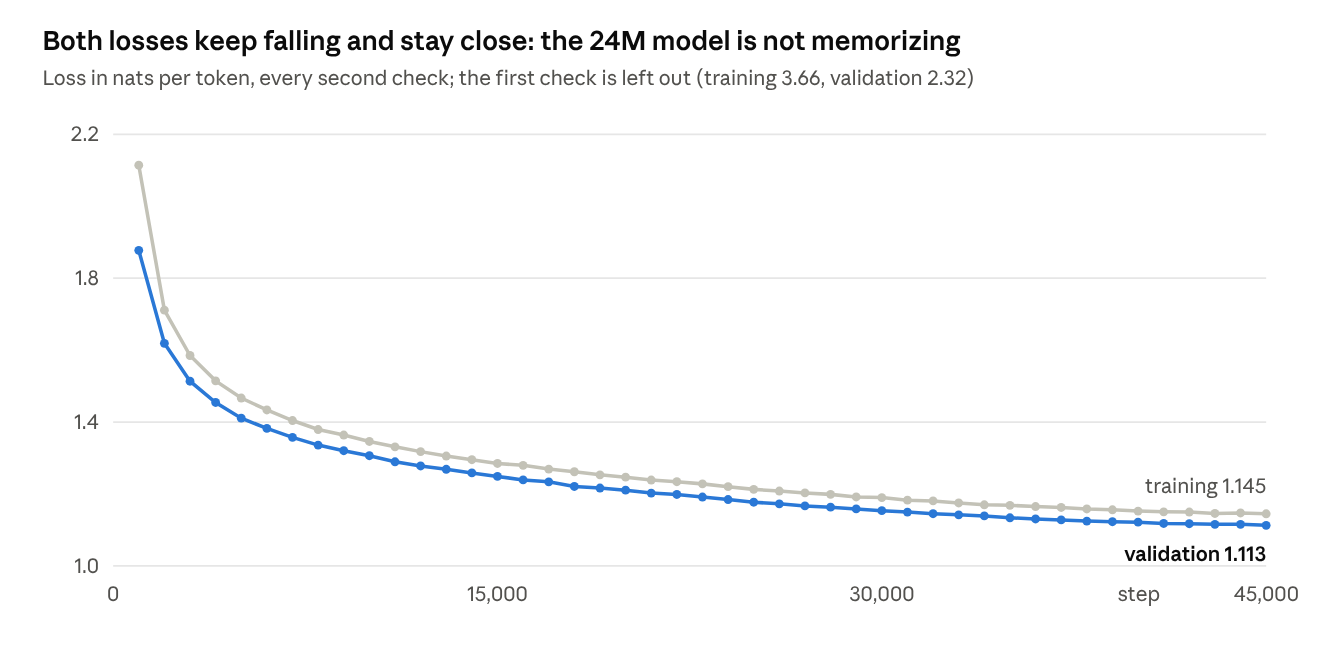
\includegraphics[width=\linewidth]{how-an-llm-works-figures/loss-curve.png}
\caption{reports/tinystories-v2-train.log $\cdot$ the medium model, 45,000 steps on TinyStories}
\end{figure}

The validation line rose at only 2 of 89 checks, and each rise was tiny. Small rises like these are noise, so read the trend.

\subsection*{Why the training line sits above validation here}
\phantomsection
\addcontentsline{toc}{subsection}{Why the training line sits above validation here}

This looks backwards, but the log explains it. Its training number is an average over the previous 500 steps, when the weights were still worse, and dropout was on. Its validation number is measured at the end of those steps, with dropout off.

To compare fairly, score both at the same checkpoint with dropout off. For this model, that gives a training loss of 1.098 and a validation loss of 1.120 on 200 windows. The gap is 0.021.

\subsection*{What overfitting looks like}
\phantomsection
\addcontentsline{toc}{subsection}{What overfitting looks like}

The same code once trained on a much smaller collection of essays. These are the real results, each measured the fair way:

{\small
\begin{longtable}{@{}>{\raggedright\arraybackslash}p{\dimexpr 0.258\linewidth-2\tabcolsep\relax}>{\raggedright\arraybackslash}p{\dimexpr 0.155\linewidth-2\tabcolsep\relax}>{\raggedright\arraybackslash}p{\dimexpr 0.206\linewidth-2\tabcolsep\relax}>{\raggedright\arraybackslash}p{\dimexpr 0.134\linewidth-2\tabcolsep\relax}>{\raggedright\arraybackslash}p{\dimexpr 0.155\linewidth-2\tabcolsep\relax}>{\raggedright\arraybackslash}p{\dimexpr 0.093\linewidth-2\tabcolsep\relax}@{}}
\toprule
\textbf{Model and data} & \textbf{Training tokens} & \textbf{Parameters per token} & \textbf{Training loss} & \textbf{Validation loss} & \textbf{Gap} \\
\midrule
\endhead
100.7M parameters, essays & 1.4M & 71.6 & 3.42 & 5.72 & 2.29 \\
15.7M parameters, essays & 1.4M & 11.2 & 4.74 & 5.61 & 0.87 \\
24.1M parameters, stories & 556M & 0.04 & 1.098 & 1.120 & 0.021 \\
\bottomrule
\end{longtable}
}

The first model has far more weights than tokens, so it can store text instead of learning general patterns. Its training loss is the best of the two essay models, but its validation loss is worse.

Notice what fixed this. The model in the last row is larger than the second one, yet its gap is far smaller, because it had about 400 times more data.

\Needspace{10\baselineskip}
\subsection*{Reading the signs}
\phantomsection
\addcontentsline{toc}{subsection}{Reading the signs}

{\small
\begin{longtable}{@{}>{\raggedright\arraybackslash}p{\dimexpr 0.225\linewidth-2\tabcolsep\relax}>{\raggedright\arraybackslash}p{\dimexpr 0.388\linewidth-2\tabcolsep\relax}>{\raggedright\arraybackslash}p{\dimexpr 0.388\linewidth-2\tabcolsep\relax}@{}}
\toprule
\textbf{What you see} & \textbf{What it usually means} & \textbf{What to try} \\
\midrule
\endhead
Training falls and validation rises & Overfitting: the model is memorizing & More data, a smaller model, more dropout, or stop at the best checkpoint \\
Both are high and flat & The model is too small, or the learning rate is wrong & A bigger model, or a different learning rate \\
Both still falling at the end & Training stopped too early & More steps \\
Loss stays near ln V & Nothing is being learned: the weights may not be updating, or inputs and targets may not line up & Try to overfit a few tokens first \\
Loss falls far too low, far too fast & The model can see the answer: targets not shifted, or the mask is missing & Run the random-token test in section 15 \\
Loss becomes NaN & Unstable steps & A lower learning rate, and check clipping \\
\bottomrule
\end{longtable}
}

The trainer keeps two files for this. \code{gpt.\allowbreak{}pt} is the latest state, used for resuming, and \code{gpt-best.\allowbreak{}pt} is the state with the lowest validation loss, used for writing text.

\subsection*{Loss is not enough}
\phantomsection
\addcontentsline{toc}{subsection}{Loss is not enough}

Loss cannot see some failures, so \code{reports/\allowbreak{}compare\_\allowbreak{}stories.\allowbreak{}py} (a local script, not in the repository) also reads the model's own writing. It generates stories and measures four things:

{\small
\begin{longtable}{@{}>{\raggedright\arraybackslash}p{\dimexpr 0.436\linewidth-2\tabcolsep\relax}>{\raggedright\arraybackslash}p{\dimexpr 0.295\linewidth-2\tabcolsep\relax}>{\raggedright\arraybackslash}p{\dimexpr 0.269\linewidth-2\tabcolsep\relax}@{}}
\toprule
\textbf{Check} & \textbf{What it catches} & \textbf{24M model, 40 stories} \\
\midrule
\endhead
Stopped at EOS & Stories that never end & 40 of 40 \\
Repeated 4-word runs & Getting stuck in a loop & 0.7\% \\
Words not in the data & Invented words & 0 \\
16-token runs copied from training & Memorized text & 5.0\% \\
\bottomrule
\end{longtable}
}

Then read some samples yourself. Numbers cannot tell you whether a story makes sense.

\section*{13. Writing text: generation}
\phantomsection
\addcontentsline{toc}{section}{13. Writing text: generation}

Writing is a loop: predict, adjust the probabilities with a few rules, sample one token, add it to the input, and repeat until EOS. The weights never change during this loop.

\Needspace{15\baselineskip}
\begin{lstlisting}[language=Python]
# model/modern_gpt.py, ModernGPT.generate (the adjustment rules come below)
self.eval()
for step in range(max_new_tokens):
    idx_cond = idx[:, -self.block_size:]       # keep only the last 768 tokens
    logits, _ = self(idx_cond)
    logits = logits[:, -1, :]                  # only the last position matters

    # ... block EOS, repetition penalty, temperature, top-k, top-p ...

    probs = F.softmax(logits, dim=-1)
    next_token = torch.multinomial(probs, 1)   # sample one token
    idx = torch.cat([idx, next_token], dim=1)

    if eos_id is not None and (next_token == eos_id).all():
        break
\end{lstlisting}

The web app in \code{web/\allowbreak{}server.\allowbreak{}py} runs its own copy of this loop, because it sends each token to the page as soon as it is made.

\subsection*{Why sample and not take the top token}
\phantomsection
\addcontentsline{toc}{subsection}{Why sample and not take the top token}

Always taking the most likely token tends to fall into repeating loops, and it gives the same text every time. Sampling keeps variety, and the rules below control how adventurous that sampling is.

\subsection*{Temperature}
\phantomsection
\addcontentsline{toc}{subsection}{Temperature}

Temperature T divides the logits before softmax. Below 1 it sharpens the distribution toward the top tokens, and above 1 it flattens it.
\[
p_j = \frac{\exp(z_j/T)}{\sum_{l}\exp(z_l/T)}
\]

Here is the real 24M model continuing “One day, a little dog” with the same random seed, changing only the temperature and using no other rule:

{\small
\begin{longtable}{@{}>{\raggedright\arraybackslash}p{\dimexpr 0.127\linewidth-2\tabcolsep\relax}>{\raggedright\arraybackslash}p{\dimexpr 0.873\linewidth-2\tabcolsep\relax}@{}}
\toprule
\textbf{T} & \textbf{Output} \\
\midrule
\endhead
0.2 & named Max went for a walk. He saw a big tree and wanted to play. Max ran to the tree and started to dig. He dug and dug until he found something shiny. \\
0.75 & named Spot went for a walk in the park. He was very filthy from playing in the mud. Spot loved to play in the mud, but today, he wanted to be clean. \\
1.5 & named Tim went out to play in the park. He arrived at filthy any floats next to the swings and dirt paveil. Tim ran slamaving his mom's chased barking, one bin stretched behind \\
3.0 & thick gorilla bumpapped rolling humble g law sail bridge mosquito arrived purp filthy exc flo noises nextged on Mum doing blackboard \\
\bottomrule
\end{longtable}
}

Low temperature is safe and plain. High temperature picks unlikely tokens, and these can join into words that do not exist, such as “paveil”, since tokens are only pieces of words.

\subsection*{Repetition penalty}
\phantomsection
\addcontentsline{toc}{subsection}{Repetition penalty}

Every token already in the context gets its logit pushed down, by a factor r of 1.08 in the app. The sign decides how, so that both cases lower the score.
\[
z_j \leftarrow \begin{cases} z_j / r & z_j \ge 0 \\ z_j \cdot r & z_j < 0 \end{cases}
\]

\subsection*{Top-k and top-p}
\phantomsection
\addcontentsline{toc}{subsection}{Top-k and top-p}

These two rules remove unlikely tokens altogether, which stops rare nonsense from slipping in.

\begin{itemize}
\item \textbf{Top-k} keeps only the k highest scores, 40 in the app.
\item \textbf{Top-p}, or nucleus sampling, sorts the tokens and keeps the smallest group whose probabilities add up to at least p, 0.92 in the app. A confident prediction keeps a few tokens, and an uncertain one keeps many.
\end{itemize}

\subsection*{All the rules on one example}
\phantomsection
\addcontentsline{toc}{subsection}{All the rules on one example}

Take six made-up tokens, where \vs{}dog and \vs{}the have already appeared. The rules run in this order, with r = 1.08, T = 0.75, k = 4 and p = 0.92. Each row shows the probabilities after that rule.

{\small
\begin{longtable}{@{}>{\raggedright\arraybackslash}p{\dimexpr 0.250\linewidth-2\tabcolsep\relax}>{\raggedright\arraybackslash}p{\dimexpr 0.125\linewidth-2\tabcolsep\relax}>{\raggedright\arraybackslash}p{\dimexpr 0.125\linewidth-2\tabcolsep\relax}>{\raggedright\arraybackslash}p{\dimexpr 0.125\linewidth-2\tabcolsep\relax}>{\raggedright\arraybackslash}p{\dimexpr 0.125\linewidth-2\tabcolsep\relax}>{\raggedright\arraybackslash}p{\dimexpr 0.125\linewidth-2\tabcolsep\relax}>{\raggedright\arraybackslash}p{\dimexpr 0.125\linewidth-2\tabcolsep\relax}@{}}
\toprule
\textbf{After this step} & \textbf{\vs{}dog} & \textbf{\vs{}cat} & \textbf{\vs{}ball} & \textbf{\vs{}tree} & \textbf{\vs{}sky} & \textbf{\vs{}the} \\
\midrule
\endhead
Raw logits & 3.0 & 2.2 & 1.5 & 0.5 & $-$0.5 & $-$1.0 \\
Softmax only & 55.5\% & 24.9\% & 12.4\% & 4.6\% & 1.7\% & 1.0\% \\
Repetition penalty & 50.0\% & 28.0\% & 13.9\% & 5.1\% & 1.9\% & 1.1\% \\
Temperature 0.75 & 58.4\% & 27.0\% & 10.6\% & 2.8\% & 0.7\% & 0.3\% \\
Top-k 4 & 59.1\% & 27.3\% & 10.8\% & 2.8\% & 0 & 0 \\
Top-p 0.92 & 60.8\% & 28.1\% & 11.1\% & 0 & 0 & 0 \\
\bottomrule
\end{longtable}
}

For top-p, the running total is 59.1\%, then 86.4\%, then 97.2\%. It passes 92\% at \vs{}ball, so \vs{}tree is dropped. The model then samples from the last row.

\subsection*{Stopping}
\phantomsection
\addcontentsline{toc}{subsection}{Stopping}

The loop ends when the model picks EOS or reaches the token limit. A prompt can look like the end of a story, so \code{min\_\allowbreak{}new\_\allowbreak{}tokens} sets EOS's logit to minus infinity for the first 20 tokens. That way the reply is never empty.

\subsection*{The context window is the model's only memory}
\phantomsection
\addcontentsline{toc}{subsection}{The context window is the model's only memory}

\code{idx[:,\allowbreak{} -self.\allowbreak{}block\_\allowbreak{}size:]} keeps the last 768 tokens and drops the rest. Whatever falls out of that window is gone completely, because the model stores nothing else between steps.

\subsection*{What a KV cache would add}
\phantomsection
\addcontentsline{toc}{subsection}{What a KV cache would add}

This code does not have a KV cache. For each new token, it reruns every block over the whole context, even though the earlier tokens' keys and values have not changed.

A KV cache would save each layer's K and V, so that each new token computes only its own Q, K and V. That is why production systems use one, and why GQA matters to them: fewer key and value heads make the cache smaller. Section 15 suggests adding one as an exercise.

\section*{14. From this model to ChatGPT}
\phantomsection
\addcontentsline{toc}{section}{14. From this model to ChatGPT}

Large assistants use the same core as this repository: tokens, embeddings, attention blocks, cross-entropy and sampling. They differ in scale, in data, and in extra training stages that teach them to respond helpfully.

\subsection*{Why this model cannot answer questions}
\phantomsection
\addcontentsline{toc}{subsection}{Why this model cannot answer questions}

Ask the 24M model to continue “The capital of France is”. Its top guesses are \vs{}a at 25.5\%, \vs{}the at 9.8\%, \vs{}not at 6.4\% and \vs{}very at 6.3\%, and \vs{}Paris is not in its top 8.

Nothing is broken. It only ever saw children's stories, so it continues text the way those stories would. Whatever an LLM “knows” comes from its training data, and that holds for the largest models too.

\subsection*{What stays the same and what changes}
\phantomsection
\addcontentsline{toc}{subsection}{What stays the same and what changes}

The right-hand column is approximate and comes from general knowledge. It was not measured here.

{\small
\begin{longtable}{@{}>{\raggedright\arraybackslash}p{\dimexpr 0.187\linewidth-2\tabcolsep\relax}>{\raggedright\arraybackslash}p{\dimexpr 0.424\linewidth-2\tabcolsep\relax}>{\raggedright\arraybackslash}p{\dimexpr 0.388\linewidth-2\tabcolsep\relax}@{}}
\toprule
\textbf{Aspect} & \textbf{This repository} & \textbf{A large production LLM} \\
\midrule
\endhead
Architecture & Decoder-only Transformer with RMSNorm, RoPE, GQA and SwiGLU & Same kind; the Llama family uses these same parts \\
Parameters & 11M to 185M & Tens to hundreds of billions \\
Vocabulary & 4,096 to 8,192 tokens & Tens of thousands to over 100,000 tokens \\
Context & 768 tokens & Many thousands of tokens or more \\
Training data & 0.56 to 1.15 billion tokens of simple stories & Trillions of tokens of varied text \\
Hardware & One RTX 3060 & Thousands of data-centre GPUs \\
KV cache & No & Yes \\
Training after pretraining & None for the story models & Instruction tuning, human feedback and safety training \\
\bottomrule
\end{longtable}
}

\subsection*{How a pretrained model becomes an assistant}
\phantomsection
\addcontentsline{toc}{subsection}{How a pretrained model becomes an assistant}

\begin{enumerate}
\item \textbf{Pretraining.} Next-token prediction on a huge amount of text. This whole guide describes this stage.
\item \textbf{Instruction tuning.} The same training loop continues at a lower learning rate, on examples of questions followed by good answers.
\item \textbf{Preference training.} People rank the model's replies, and training moves it toward the replies they preferred.
\item \textbf{Retrieval and tools.} Around the model, software finds documents and places them in the prompt, so the model can read facts it was never trained on.
\end{enumerate}

The key idea is that a chat is just a document. The system writes the conversation as tokens, ends at the point where the assistant's turn begins, and asks for the next token. Even then, the model is only continuing text.

\subsection*{The closest parts in this repository}
\phantomsection
\addcontentsline{toc}{subsection}{The closest parts in this repository}

\begin{itemize}
\item \textbf{Continued training.} \code{--mode update} in \code{training/\allowbreak{}train.\allowbreak{}py}, run through \code{pipeline/\allowbreak{}learn.\allowbreak{}py}, restarts from the best checkpoint at a lower learning rate (6e-5). Each batch has a 35\% chance of coming from older data. This replay stops the model from forgetting what it knew while it learns new material.
\item \textbf{Retrieval.} \code{rag.\allowbreak{}py} finds matching text, and \code{web/\allowbreak{}server.\allowbreak{}py} can place it in a prompt with SOURCE, QUESTION and ANSWER labels. The story models never saw that format, so they would treat it as strange text and not use it as an answer source.
\end{itemize}

\subsection*{Limits that follow from how it works}
\phantomsection
\addcontentsline{toc}{subsection}{Limits that follow from how it works}

\begin{itemize}
\item \textbf{It predicts and does not look things up.} There is no table of facts inside, so a false sentence can score as likely as a true one. Asked about France, this model wrote a story with invented words such as “capination”.
\item \textbf{Probability is not confidence in truth.} A high probability means the text is likely to come next, not that it is correct.
\item \textbf{It does not learn while you use it.} The weights are fixed once training ends.
\item \textbf{It remembers only its context window.} Anything before the last 768 tokens is gone.
\item \textbf{Answers vary.} Sampling is random, so the same prompt gives different text unless the seed is fixed.
\item \textbf{More size cannot replace missing data.} A bigger model trained only on stories can get better at stories, but it still cannot learn facts that the stories do not contain.
\end{itemize}

\section*{15. Experiments to try}
\phantomsection
\addcontentsline{toc}{section}{15. Experiments to try}

The fastest way to understand this code is to test its claims yourself. All the Python below was run on the trained 24M model, and most of it runs on a CPU in seconds.

\subsection*{Setup}
\phantomsection
\addcontentsline{toc}{subsection}{Setup}

Checkpoints are not stored in git, so train a small model first. On an RTX 3060, the \code{small} profile took about 1.4 hours for 20,000 steps on TinyStories.

\Needspace{3\baselineskip}
\begin{lstlisting}[language=bash]
python -m dataset.large_text --train path/to/train.txt --val path/to/valid.txt --out data/mydata
\end{lstlisting}

\Needspace{3\baselineskip}
\begin{lstlisting}[language=bash]
python -m training.train --model-size small --data-dir data/mydata --checkpoint-dir checkpoints/my-run --eval-interval 500 --steps 20000
\end{lstlisting}

Then load it in Python:

\Needspace{11\baselineskip}
\begin{lstlisting}[language=Python]
import torch
import torch.nn.functional as F
from model.modern_gpt import ModernGPT
from tokenizer.bpe import BPETokenizer

ck = torch.load("checkpoints/my-run/gpt-best.pt", map_location="cpu", weights_only=False)
model = ModernGPT(**ck["config"])
model.load_state_dict(ck["model_state"])
model.eval()
tok = BPETokenizer.load("data/mydata/vocab.json")
\end{lstlisting}

\subsection*{1. See the tokens}
\phantomsection
\addcontentsline{toc}{subsection}{1. See the tokens}

Try rare words, numbers and other languages. How many tokens does each take?

\Needspace{4\baselineskip}
\begin{lstlisting}[language=Python]
ids = tok.encode("Once upon a time, a little dog found a red ball.")
print([tok.decode([i]) for i in ids])
\end{lstlisting}

\subsection*{2. See the next-token probabilities}
\phantomsection
\addcontentsline{toc}{subsection}{2. See the next-token probabilities}

Change the prompt by one word and watch the list move.

\Needspace{8\baselineskip}
\begin{lstlisting}[language=Python]
ids = tok.encode("Lily was very")
with torch.no_grad():
    logits, _ = model(torch.tensor([ids]))
top = logits[0, -1].softmax(-1).topk(8)
for p, i in zip(top.values, top.indices):
    print(repr(tok.decode([int(i)])), round(float(p), 3))
\end{lstlisting}

\subsection*{3. Prove the mask works}
\phantomsection
\addcontentsline{toc}{subsection}{3. Prove the mask works}

Change one token and see which scores change. The first 5 printed values should be exactly 0.

\Needspace{9\baselineskip}
\begin{lstlisting}[language=Python]
ids = tok.encode("Once upon a time, there was a little dog named Max.")
a = torch.tensor([ids])
b = a.clone()
b[0, 5] = tok.encode(" cat")[0]
with torch.no_grad():
    la, _ = model(a)
    lb, _ = model(b)
print((la - lb).abs().amax(dim=(0, 2)))
\end{lstlisting}

\subsection*{4. Explore the embeddings}
\phantomsection
\addcontentsline{toc}{subsection}{4. Explore the embeddings}

Try colours, numbers, names and verbs.

\Needspace{6\baselineskip}
\begin{lstlisting}[language=Python]
E = F.normalize(model.embedding.weight.detach(), dim=-1)
i = tok.encode(" dog")[0]
top = (E @ E[i]).topk(6)
print([tok.decode([int(j)]) for j in top.indices[1:]])
\end{lstlisting}

\subsection*{5. Feel the temperature}
\phantomsection
\addcontentsline{toc}{subsection}{5. Feel the temperature}

Run this at 0.2, 0.75, 1.5 and 3.0. Setting top-k to 0 and top-p to 1.0 turns those two rules off.

\Needspace{3\baselineskip}
\begin{lstlisting}[language=bash]
python -m generation.generate --checkpoint checkpoints/my-run/gpt-best.pt --data-dir data/mydata --prompt "One day, a little dog" --temperature 1.5 --top-k 0 --top-p 1.0 --repetition-penalty 1.0
\end{lstlisting}

\subsection*{6. Catch a model that can see the answer}
\phantomsection
\addcontentsline{toc}{subsection}{6. Catch a model that can see the answer}

Random tokens cannot be predicted, so an honest model's loss must stay at the natural log of the number of possible tokens. Here that is ln 252 = 5.53. This test needs no checkpoint or data.

\Needspace{20\baselineskip}
\begin{lstlisting}[language=Python]
import torch
from model.modern_gpt import ModernGPT

cfg = dict(vocab_size=256, block_size=32, dim=64, n_layers=2, n_heads=4,
           n_kv_heads=2, ffn_dim=170, dropout=0.0)

def run(shift=1, steps=800):
    torch.manual_seed(1)
    model = ModernGPT(**cfg)
    opt = torch.optim.AdamW(model.parameters(), lr=1e-3)
    for _ in range(steps):
        tokens = torch.randint(4, 256, (16, 34))     # new random tokens every step
        x, y = tokens[:, :32], tokens[:, shift:32 + shift]
        _, loss = model(x, y)
        opt.zero_grad(set_to_none=True)
        loss.backward()
        opt.step()
    return loss.item()

print("normal", run())
print("not shifted", run(shift=0))
\end{lstlisting}

To test the mask, change \code{is\_\allowbreak{}causal=True} to \code{False} in \code{GQAAttention.\allowbreak{}forward} and run it again, then change it back. These are the measured results, averaged over the last 50 steps:

{\small
\begin{longtable}{@{}>{\raggedright\arraybackslash}p{\dimexpr 0.202\linewidth-2\tabcolsep\relax}>{\raggedright\arraybackslash}p{\dimexpr 0.213\linewidth-2\tabcolsep\relax}>{\raggedright\arraybackslash}p{\dimexpr 0.585\linewidth-2\tabcolsep\relax}@{}}
\toprule
\textbf{Run} & \textbf{Loss after 800 steps} & \textbf{What it means} \\
\midrule
\endhead
Normal & 5.53 & Correct: nothing can be predicted \\
Targets not shifted & 0.007 & The answer is at the same position in the input \\
Mask removed & 0.20 & The model learned to read the next token from its input \\
\bottomrule
\end{longtable}
}

A loss near 0 on random data is impossible without seeing the answer. Keep this test in mind for any change you make to the model.

\subsection*{7. Change the model and predict first}
\phantomsection
\addcontentsline{toc}{subsection}{7. Change the model and predict first}

These have no measured answer here. Write down what you expect before running each one, on the same data and for the same number of steps.

\begin{itemize}
\item \textbf{Remove RoPE:} delete the \code{apply\_\allowbreak{}rope} line. Word order becomes much harder, so expect a higher validation loss.
\item \textbf{Remove the scaling:} use your own attention without the square root of $d_k$, using the five lines from section 5.
\item \textbf{Use standard attention:} set \code{n\_\allowbreak{}kv\_\allowbreak{}heads} equal to \code{n\_\allowbreak{}heads}. How much validation loss do the 25M extra parameters buy?
\item \textbf{Remove the residual connections:} write \code{x = self.\allowbreak{}attention(self.\allowbreak{}norm1(x))}. Does a deep model still train?
\item \textbf{Change the data size:} train on 1\% of the tokens, and watch the gap between training and validation.
\end{itemize}

\subsection*{8. Bigger exercise: add a KV cache}
\phantomsection
\addcontentsline{toc}{subsection}{8. Bigger exercise: add a KV cache}

Store each layer's K and V between steps, so that each new token computes only its own Q, K and V. RoPE needs the true position of the new token, and the cache must be cut when the window passes 768 tokens.

You can check your work easily. With a context below 768 tokens and the same seed, the cached version should produce the same text as today's \code{generate}, only faster.

\newpage

\section*{Papers behind each idea}
\phantomsection
\addcontentsline{toc}{section}{Papers behind each idea}

Each link goes to the paper on arXiv.

{\small
\begin{longtable}{@{}>{\raggedright\arraybackslash}p{\dimexpr 0.330\linewidth-2\tabcolsep\relax}>{\raggedright\arraybackslash}p{\dimexpr 0.670\linewidth-2\tabcolsep\relax}@{}}
\toprule
\textbf{Idea} & \textbf{Paper} \\
\midrule
\endhead
Transformer and attention & \href{https://arxiv.org/abs/1706.03762}{Attention Is All You Need} \\
BPE for language & \href{https://arxiv.org/abs/1508.07909}{Neural Machine Translation of Rare Words with Subword Units} \\
RoPE & \href{https://arxiv.org/abs/2104.09864}{RoFormer: Enhanced Transformer with Rotary Position Embedding} \\
RMSNorm & \href{https://arxiv.org/abs/1910.07467}{Root Mean Square Layer Normalization} \\
SwiGLU & \href{https://arxiv.org/abs/2002.05202}{GLU Variants Improve Transformer} \\
Grouped-query attention & \href{https://arxiv.org/abs/2305.13245}{GQA: Training Generalized Multi-Query Transformer Models from Multi-Head Checkpoints} \\
AdamW & \href{https://arxiv.org/abs/1711.05101}{Decoupled Weight Decay Regularization} \\
Top-p sampling & \href{https://arxiv.org/abs/1904.09751}{The Curious Case of Neural Text Degeneration} \\
Instruction and preference training & \href{https://arxiv.org/abs/2203.02155}{Training language models to follow instructions with human feedback} \\
A production model with these parts & \href{https://arxiv.org/abs/2307.09288}{Llama 2: Open Foundation and Fine-Tuned Chat Models} \\
The story data & \href{https://arxiv.org/abs/2305.07759}{TinyStories} and \href{https://arxiv.org/abs/2504.09184}{SimpleStories} \\
\bottomrule
\end{longtable}
}

\end{document}
